\documentclass[11pt,a4paper]{article}
\usepackage[margin=2.4cm]{geometry}
% Shared preamble of the manuscript and the extended abstract.
\usepackage[T1]{fontenc}
\usepackage[utf8]{inputenc}
\usepackage[spanish,es-noshorthands,es-tabla]{babel}
\usepackage{lmodern}
\usepackage{microtype}
\usepackage{amsmath,amssymb}
\usepackage[separate-uncertainty=true,group-separator={\,},output-decimal-marker={,},per-mode=symbol]{siunitx}
\usepackage{graphicx}
\usepackage{booktabs}
\usepackage{threeparttable}
\usepackage{tabularx}
\usepackage{caption}
\captionsetup{font=small,labelfont=bf}
\usepackage{xcolor}
\usepackage{tikz}
\usetikzlibrary{positioning,arrows.meta,fit,backgrounds}
\usepackage{csquotes}
\usepackage[backend=biber,style=authoryear,maxcitenames=2,maxbibnames=10,uniquelist=false,uniquename=false,giveninits=true,doi=true,url=false,isbn=false]{biblatex}
\DeclareFieldFormat[article]{title}{#1}
\usepackage[hidelinks]{hyperref}
\graphicspath{{../results/figures/}}
\sisetup{round-mode=places,round-precision=2}
\newcommand{\ETa}{\mathrm{ET_a}}
\newcommand{\ETr}{\mathrm{ET_r}}
\newcommand{\ETrF}{\mathrm{ET_rF}}
\newcommand{\Rn}{R_n}
\newcommand{\pkg}[1]{\textsf{#1}}
\newcommand{\code}[1]{\texttt{#1}}

\addbibresource{../references/references.bib}
% Generated by scripts/08_numbers.R - do not edit by hand.
\newcommand{\EarthFluxVersion}{0.1.0.9000}
\newcommand{\EarthFluxCommit}{95d3175}
\newcommand{\Seed}{20270121}
\newcommand{\NMC}{200}
\newcommand{\NTests}{614}
\newcommand{\NExpectations}{4.473}
\newcommand{\NTestsFailed}{0}
\newcommand{\NTestsError}{17}
\newcommand{\NTestsSkipped}{9}
\newcommand{\NTestsPassed}{588}
\newcommand{\NExports}{73}
\newcommand{\NLinesR}{24.027}
\newcommand{\NDecisions}{17}
\newcommand{\VerRows}{49}
\newcommand{\VerVerified}{31}
\newcommand{\VerCorroborated}{3}
\newcommand{\VerCandidate}{9}
\newcommand{\VerDiscrepancies}{7}
\newcommand{\VerFixed}{2}
\newcommand{\SceneElevMax}{863}
\newcommand{\SceneCellsProvince}{3.779}
\newcommand{\SceneCellsValid}{3.653}
\newcommand{\NStations}{63}
\newcommand{\NStationsDMC}{5}
\newcommand{\NStationsINIA}{21}
\newcommand{\NStationsFDF}{35}
\newcommand{\NStationsISD}{2}
\newcommand{\NStationsWind}{7}
\newcommand{\RepStationName}{General Bernardo O'Higgins, Chillán Ad.}
\newcommand{\RepStationDist}{80}
\newcommand{\NCVDays}{90}
\newcommand{\NFolds}{17}
\newcommand{\NCVPred}{51.705}
\newcommand{\CVTaCOneRmse}{2,70}
\newcommand{\CVTaCOneRmseLo}{2,57}
\newcommand{\CVTaCOneRmseHi}{2,84}
\newcommand{\CVTaCOneBias}{-0,16}
\newcommand{\CVTaCOneR}{0,70}
\newcommand{\CVTaCOneFailed}{0}
\newcommand{\CVTaCOneN}{5.498}
\newcommand{\CVTaCOneLapRmse}{2,77}
\newcommand{\CVTaCOneLapRmseLo}{2,64}
\newcommand{\CVTaCOneLapRmseHi}{2,90}
\newcommand{\CVTaCOneLapBias}{-0,05}
\newcommand{\CVTaCOneLapR}{0,68}
\newcommand{\CVTaCOneLapFailed}{0}
\newcommand{\CVTaCOneLapN}{5.498}
\newcommand{\CVTaCTwoIDWRmse}{2,32}
\newcommand{\CVTaCTwoIDWRmseLo}{2,22}
\newcommand{\CVTaCTwoIDWRmseHi}{2,42}
\newcommand{\CVTaCTwoIDWBias}{0,01}
\newcommand{\CVTaCTwoIDWR}{0,78}
\newcommand{\CVTaCTwoIDWFailed}{0}
\newcommand{\CVTaCTwoIDWN}{5.588}
\newcommand{\CVTaCTwoOLSRmse}{2,46}
\newcommand{\CVTaCTwoOLSRmseLo}{2,36}
\newcommand{\CVTaCTwoOLSRmseHi}{2,57}
\newcommand{\CVTaCTwoOLSBias}{-0,01}
\newcommand{\CVTaCTwoOLSR}{0,75}
\newcommand{\CVTaCTwoOLSFailed}{0}
\newcommand{\CVTaCTwoOLSN}{5.588}
\newcommand{\CVTaCThreeGWRRmse}{2,40}
\newcommand{\CVTaCThreeGWRRmseLo}{2,29}
\newcommand{\CVTaCThreeGWRRmseHi}{2,51}
\newcommand{\CVTaCThreeGWRBias}{-0,04}
\newcommand{\CVTaCThreeGWRR}{0,76}
\newcommand{\CVTaCThreeGWRFailed}{0}
\newcommand{\CVTaCThreeGWRN}{5.588}
\newcommand{\CVEaCOneRmse}{0,209}
\newcommand{\CVEaCOneRmseLo}{0,195}
\newcommand{\CVEaCOneRmseHi}{0,222}
\newcommand{\CVEaCOneBias}{-0,024}
\newcommand{\CVEaCOneR}{0,69}
\newcommand{\CVEaCOneFailed}{0}
\newcommand{\CVEaCOneN}{5.495}
\newcommand{\CVEaCTwoIDWRmse}{0,169}
\newcommand{\CVEaCTwoIDWRmseLo}{0,161}
\newcommand{\CVEaCTwoIDWRmseHi}{0,178}
\newcommand{\CVEaCTwoIDWBias}{-0,005}
\newcommand{\CVEaCTwoIDWR}{0,79}
\newcommand{\CVEaCTwoIDWFailed}{0}
\newcommand{\CVEaCTwoIDWN}{5.585}
\newcommand{\CVEaCTwoOLSRmse}{0,188}
\newcommand{\CVEaCTwoOLSRmseLo}{0,178}
\newcommand{\CVEaCTwoOLSRmseHi}{0,198}
\newcommand{\CVEaCTwoOLSBias}{0,003}
\newcommand{\CVEaCTwoOLSR}{0,73}
\newcommand{\CVEaCTwoOLSFailed}{0}
\newcommand{\CVEaCTwoOLSN}{5.585}
\newcommand{\CVEaCThreeGWRRmse}{0,174}
\newcommand{\CVEaCThreeGWRRmseLo}{0,166}
\newcommand{\CVEaCThreeGWRRmseHi}{0,184}
\newcommand{\CVEaCThreeGWRBias}{-0,002}
\newcommand{\CVEaCThreeGWRR}{0,77}
\newcommand{\CVEaCThreeGWRFailed}{0}
\newcommand{\CVEaCThreeGWRN}{5.585}
\newcommand{\CVWindCOneRmse}{1,51}
\newcommand{\CVWindCOneRmseLo}{1,37}
\newcommand{\CVWindCOneRmseHi}{1,64}
\newcommand{\CVWindCOneBias}{0,63}
\newcommand{\CVWindCOneR}{0,52}
\newcommand{\CVWindCOneFailed}{0}
\newcommand{\CVWindCOneN}{505}
\newcommand{\CVWindCTwoIDWRmse}{1,19}
\newcommand{\CVWindCTwoIDWRmseLo}{1,10}
\newcommand{\CVWindCTwoIDWRmseHi}{1,29}
\newcommand{\CVWindCTwoIDWBias}{-0,04}
\newcommand{\CVWindCTwoIDWR}{0,58}
\newcommand{\CVWindCTwoIDWFailed}{0}
\newcommand{\CVWindCTwoIDWN}{595}
\newcommand{\CVWindCTwoOLSRmse}{7,39}
\newcommand{\CVWindCTwoOLSRmseLo}{1,48}
\newcommand{\CVWindCTwoOLSRmseHi}{12,69}
\newcommand{\CVWindCTwoOLSBias}{0,10}
\newcommand{\CVWindCTwoOLSR}{0,08}
\newcommand{\CVWindCTwoOLSFailed}{0}
\newcommand{\CVWindCTwoOLSN}{595}
\newcommand{\PairTaCOneDse}{-1,491}
\newcommand{\PairTaCOneLo}{-2,022}
\newcommand{\PairTaCOneHi}{-1,023}
\newcommand{\PairTaCOneShare}{57}
\newcommand{\PairTaCOneLapDse}{-1,852}
\newcommand{\PairTaCOneLapLo}{-2,393}
\newcommand{\PairTaCOneLapHi}{-1,341}
\newcommand{\PairTaCOneLapShare}{58}
\newcommand{\PairTaCTwoOLSDse}{-0,302}
\newcommand{\PairTaCTwoOLSLo}{-0,526}
\newcommand{\PairTaCTwoOLSHi}{-0,096}
\newcommand{\PairTaCTwoOLSShare}{55}
\newcommand{\PairTaCTwoIDWDse}{0,366}
\newcommand{\PairTaCTwoIDWLo}{0,187}
\newcommand{\PairTaCTwoIDWHi}{0,554}
\newcommand{\PairTaCTwoIDWShare}{51}
\newcommand{\PairEaCOneDse}{-0,0127}
\newcommand{\PairEaCOneLo}{-0,0175}
\newcommand{\PairEaCOneHi}{-0,0088}
\newcommand{\PairEaCOneShare}{61}
\newcommand{\PairEaCTwoOLSDse}{-0,0048}
\newcommand{\PairEaCTwoOLSLo}{-0,0068}
\newcommand{\PairEaCTwoOLSHi}{-0,0030}
\newcommand{\PairEaCTwoOLSShare}{59}
\newcommand{\PairEaCTwoIDWDse}{0,0018}
\newcommand{\PairEaCTwoIDWLo}{0,0011}
\newcommand{\PairEaCTwoIDWHi}{0,0025}
\newcommand{\PairEaCTwoIDWShare}{48}
\newcommand{\CVWindCThreeGWRFailed}{595}
\newcommand{\CVWindCThreeGWRTotal}{595}
\newcommand{\CVWindOLSMax}{178}
\newcommand{\CVWindOLSNeg}{47}
\newcommand{\MoranTaCOneI}{0,14}
\newcommand{\MoranTaCOneSig}{74}
\newcommand{\MoranEaCOneI}{0,12}
\newcommand{\MoranEaCOneSig}{82}
\newcommand{\MoranTaCOneLapI}{0,14}
\newcommand{\MoranTaCOneLapSig}{77}
\newcommand{\MoranTaCTwoIDWI}{-0,00}
\newcommand{\MoranTaCTwoIDWSig}{1}
\newcommand{\MoranEaCTwoIDWI}{0,02}
\newcommand{\MoranEaCTwoIDWSig}{22}
\newcommand{\MoranTaCTwoOLSI}{0,13}
\newcommand{\MoranTaCTwoOLSSig}{70}
\newcommand{\MoranEaCTwoOLSI}{0,14}
\newcommand{\MoranEaCTwoOLSSig}{83}
\newcommand{\MoranTaCThreeGWRI}{0,01}
\newcommand{\MoranTaCThreeGWRSig}{13}
\newcommand{\MoranEaCThreeGWRI}{0,04}
\newcommand{\MoranEaCThreeGWRSig}{38}
\newcommand{\DensTaCTwoIDWQuarter}{2,39}
\newcommand{\DensTaCTwoIDWQuarterN}{16}
\newcommand{\DensEaCTwoIDWQuarter}{0,155}
\newcommand{\DensEaCTwoIDWQuarterN}{16}
\newcommand{\DensTaCTwoIDWHalf}{2,39}
\newcommand{\DensTaCTwoIDWHalfN}{32}
\newcommand{\DensEaCTwoIDWHalf}{0,166}
\newcommand{\DensEaCTwoIDWHalfN}{32}
\newcommand{\DensTaCTwoIDWThreeQ}{2,29}
\newcommand{\DensTaCTwoIDWThreeQN}{47}
\newcommand{\DensEaCTwoIDWThreeQ}{0,171}
\newcommand{\DensEaCTwoIDWThreeQN}{47}
\newcommand{\DensTaCTwoIDWAll}{2,30}
\newcommand{\DensTaCTwoIDWAllN}{63}
\newcommand{\DensEaCTwoIDWAll}{0,170}
\newcommand{\DensEaCTwoIDWAllN}{63}
\newcommand{\DensTaCTwoOLSQuarter}{2,64}
\newcommand{\DensTaCTwoOLSQuarterN}{16}
\newcommand{\DensEaCTwoOLSQuarter}{0,182}
\newcommand{\DensEaCTwoOLSQuarterN}{16}
\newcommand{\DensTaCTwoOLSHalf}{2,53}
\newcommand{\DensTaCTwoOLSHalfN}{32}
\newcommand{\DensEaCTwoOLSHalf}{0,182}
\newcommand{\DensEaCTwoOLSHalfN}{32}
\newcommand{\DensTaCTwoOLSThreeQ}{2,42}
\newcommand{\DensTaCTwoOLSThreeQN}{47}
\newcommand{\DensEaCTwoOLSThreeQ}{0,187}
\newcommand{\DensEaCTwoOLSThreeQN}{47}
\newcommand{\DensTaCTwoOLSAll}{2,40}
\newcommand{\DensTaCTwoOLSAllN}{63}
\newcommand{\DensEaCTwoOLSAll}{0,187}
\newcommand{\DensEaCTwoOLSAllN}{63}
\newcommand{\DensTaCThreeGWRQuarter}{2,61}
\newcommand{\DensTaCThreeGWRQuarterN}{16}
\newcommand{\DensEaCThreeGWRQuarter}{0,178}
\newcommand{\DensEaCThreeGWRQuarterN}{16}
\newcommand{\DensTaCThreeGWRHalf}{2,56}
\newcommand{\DensTaCThreeGWRHalfN}{32}
\newcommand{\DensEaCThreeGWRHalf}{0,177}
\newcommand{\DensEaCThreeGWRHalfN}{32}
\newcommand{\DensTaCThreeGWRThreeQ}{2,39}
\newcommand{\DensTaCThreeGWRThreeQN}{47}
\newcommand{\DensEaCThreeGWRThreeQ}{0,182}
\newcommand{\DensEaCThreeGWRThreeQN}{47}
\newcommand{\DensTaCThreeGWRAll}{2,39}
\newcommand{\DensTaCThreeGWRAllN}{63}
\newcommand{\DensEaCThreeGWRAll}{0,177}
\newcommand{\DensEaCThreeGWRAllN}{63}
\newcommand{\OLSWindOOD}{53.511}
\newcommand{\MRnCOneMean}{475}
\newcommand{\MRnCOneSd}{55}
\newcommand{\MGCOneMean}{58}
\newcommand{\MGCOneSd}{15}
\newcommand{\MHCOneMean}{267}
\newcommand{\MHCOneSd}{73}
\newcommand{\MLECOneMean}{149}
\newcommand{\MLECOneSd}{135}
\newcommand{\MEtrfCOneMean}{0,40}
\newcommand{\MEtrfCOneSd}{0,36}
\newcommand{\MEtaCOneMean}{3,45}
\newcommand{\MEtaCOneSd}{3,12}
\newcommand{\MFTaCOneMean}{23,90}
\newcommand{\MFTaCOneSd}{0,00}
\newcommand{\MFEaCOneMean}{1,59}
\newcommand{\MFEaCOneSd}{0,00}
\newcommand{\MFWindCOneMean}{1,54}
\newcommand{\MFWindCOneSd}{0,00}
\newcommand{\MFEtrInstCOneMean}{0,546}
\newcommand{\MFEtrInstCOneSd}{0,002}
\newcommand{\MFEtrDayCOneMean}{8,56}
\newcommand{\MFEtrDayCOneSd}{0,01}
\newcommand{\MRnCOneLapMean}{477}
\newcommand{\MRnCOneLapSd}{56}
\newcommand{\MGCOneLapMean}{59}
\newcommand{\MGCOneLapSd}{15}
\newcommand{\MHCOneLapMean}{266}
\newcommand{\MHCOneLapSd}{74}
\newcommand{\MLECOneLapMean}{153}
\newcommand{\MLECOneLapSd}{137}
\newcommand{\MEtrfCOneLapMean}{0,40}
\newcommand{\MEtrfCOneLapSd}{0,37}
\newcommand{\MEtaCOneLapMean}{3,54}
\newcommand{\MEtaCOneLapSd}{3,17}
\newcommand{\MFTaCOneLapMean}{24,41}
\newcommand{\MFTaCOneLapSd}{0,85}
\newcommand{\MFEaCOneLapMean}{1,59}
\newcommand{\MFEaCOneLapSd}{0,00}
\newcommand{\MFWindCOneLapMean}{1,54}
\newcommand{\MFWindCOneLapSd}{0,00}
\newcommand{\MFEtrInstCOneLapMean}{0,554}
\newcommand{\MFEtrInstCOneLapSd}{0,016}
\newcommand{\MFEtrDayCOneLapMean}{8,72}
\newcommand{\MFEtrDayCOneLapSd}{0,26}
\newcommand{\MRnCTwoOLSMean}{449}
\newcommand{\MRnCTwoOLSSd}{62}
\newcommand{\MGCTwoOLSMean}{66}
\newcommand{\MGCTwoOLSSd}{10}
\newcommand{\MHCTwoOLSMean}{325}
\newcommand{\MHCTwoOLSSd}{31}
\newcommand{\MLECTwoOLSMean}{58}
\newcommand{\MLECTwoOLSSd}{87}
\newcommand{\MEtrfCTwoOLSMean}{0,15}
\newcommand{\MEtrfCTwoOLSSd}{0,23}
\newcommand{\MEtaCTwoOLSMean}{1,04}
\newcommand{\MEtaCTwoOLSSd}{1,51}
\newcommand{\MFTaCTwoOLSMean}{22,49}
\newcommand{\MFTaCTwoOLSSd}{0,51}
\newcommand{\MFEaCTwoOLSMean}{1,60}
\newcommand{\MFEaCTwoOLSSd}{0,03}
\newcommand{\MFWindCTwoOLSMean}{3,30}
\newcommand{\MFWindCTwoOLSSd}{0,53}
\newcommand{\MFEtrInstCTwoOLSMean}{0,567}
\newcommand{\MFEtrInstCTwoOLSSd}{0,003}
\newcommand{\MFEtrDayCTwoOLSMean}{6,95}
\newcommand{\MFEtrDayCTwoOLSSd}{0,30}
\newcommand{\MRnCTwoIDWMean}{478}
\newcommand{\MRnCTwoIDWSd}{49}
\newcommand{\MGCTwoIDWMean}{59}
\newcommand{\MGCTwoIDWSd}{16}
\newcommand{\MHCTwoIDWMean}{278}
\newcommand{\MHCTwoIDWSd}{79}
\newcommand{\MLECTwoIDWMean}{140}
\newcommand{\MLECTwoIDWSd}{133}
\newcommand{\MEtrfCTwoIDWMean}{0,37}
\newcommand{\MEtrfCTwoIDWSd}{0,38}
\newcommand{\MEtaCTwoIDWMean}{2,48}
\newcommand{\MEtaCTwoIDWSd}{2,26}
\newcommand{\MFTaCTwoIDWMean}{24,51}
\newcommand{\MFTaCTwoIDWSd}{1,92}
\newcommand{\MFEaCTwoIDWMean}{1,59}
\newcommand{\MFEaCTwoIDWSd}{0,03}
\newcommand{\MFWindCTwoIDWMean}{2,27}
\newcommand{\MFWindCTwoIDWSd}{0,07}
\newcommand{\MFEtrInstCTwoIDWMean}{0,587}
\newcommand{\MFEtrInstCTwoIDWSd}{0,045}
\newcommand{\MFEtrDayCTwoIDWMean}{7,38}
\newcommand{\MFEtrDayCTwoIDWSd}{0,86}
\newcommand{\MRnCThreeGWRMean}{483}
\newcommand{\MRnCThreeGWRSd}{54}
\newcommand{\MGCThreeGWRMean}{59}
\newcommand{\MGCThreeGWRSd}{15}
\newcommand{\MHCThreeGWRMean}{271}
\newcommand{\MHCThreeGWRSd}{72}
\newcommand{\MLECThreeGWRMean}{152}
\newcommand{\MLECThreeGWRSd}{132}
\newcommand{\MEtrfCThreeGWRMean}{0,40}
\newcommand{\MEtrfCThreeGWRSd}{0,37}
\newcommand{\MEtaCThreeGWRMean}{2,76}
\newcommand{\MEtaCThreeGWRSd}{2,25}
\newcommand{\MFTaCThreeGWRMean}{25,46}
\newcommand{\MFTaCThreeGWRSd}{2,18}
\newcommand{\MFEaCThreeGWRMean}{1,55}
\newcommand{\MFEaCThreeGWRSd}{0,04}
\newcommand{\MFWindCThreeGWRMean}{1,54}
\newcommand{\MFWindCThreeGWRSd}{0,00}
\newcommand{\MFEtrInstCThreeGWRMean}{0,574}
\newcommand{\MFEtrInstCThreeGWRSd}{0,037}
\newcommand{\MFEtrDayCThreeGWRMean}{7,56}
\newcommand{\MFEtrDayCThreeGWRSd}{0,85}
\newcommand{\CalCOneA}{-65,73}
\newcommand{\CalCOneB}{0,231}
\newcommand{\CalCOneIter}{9}
\newcommand{\CalCOneNeg}{77}
\newcommand{\CalCOneLapA}{-67,00}
\newcommand{\CalCOneLapB}{0,236}
\newcommand{\CalCOneLapIter}{9}
\newcommand{\CalCOneLapNeg}{74}
\newcommand{\CalCTwoOLSA}{-30,77}
\newcommand{\CalCTwoOLSB}{0,115}
\newcommand{\CalCTwoOLSIter}{6}
\newcommand{\CalCTwoOLSNeg}{156}
\newcommand{\CalCTwoIDWA}{-73,83}
\newcommand{\CalCTwoIDWB}{0,258}
\newcommand{\CalCTwoIDWIter}{7}
\newcommand{\CalCTwoIDWNeg}{102}
\newcommand{\CalCThreeGWRA}{-64,94}
\newcommand{\CalCThreeGWRB}{0,229}
\newcommand{\CalCThreeGWRIter}{9}
\newcommand{\CalCThreeGWRNeg}{58}
\newcommand{\CalOatTaA}{-67,46}
\newcommand{\CalOatTaB}{0,237}
\newcommand{\CalOatTaIter}{9}
\newcommand{\CalOatTaNeg}{59}
\newcommand{\CalOatEaA}{-65,25}
\newcommand{\CalOatEaB}{0,230}
\newcommand{\CalOatEaIter}{9}
\newcommand{\CalOatEaNeg}{76}
\newcommand{\CalOatWindA}{-71,51}
\newcommand{\CalOatWindB}{0,250}
\newcommand{\CalOatWindIter}{7}
\newcommand{\CalOatWindNeg}{97}
\newcommand{\CalOatEtrInstA}{-63,77}
\newcommand{\CalOatEtrInstB}{0,225}
\newcommand{\CalOatEtrInstIter}{9}
\newcommand{\CalOatEtrInstNeg}{77}
\newcommand{\CalOatEtrDayA}{-65,73}
\newcommand{\CalOatEtrDayB}{0,231}
\newcommand{\CalOatEtrDayIter}{9}
\newcommand{\CalOatEtrDayNeg}{77}
\newcommand{\RangeTaCOneAbove}{0,0}
\newcommand{\RangeTaCOneMax}{23,9}
\newcommand{\RangeTaCOneObsMax}{28,4}
\newcommand{\RangeEaCOneAbove}{0,0}
\newcommand{\RangeEaCOneMax}{1,6}
\newcommand{\RangeEaCOneObsMax}{2,0}
\newcommand{\RangeTaCOneLapAbove}{0,0}
\newcommand{\RangeTaCOneLapMax}{27,6}
\newcommand{\RangeTaCOneLapObsMax}{28,4}
\newcommand{\RangeEaCOneLapAbove}{0,0}
\newcommand{\RangeEaCOneLapMax}{1,6}
\newcommand{\RangeEaCOneLapObsMax}{2,0}
\newcommand{\RangeTaCTwoOLSAbove}{0,0}
\newcommand{\RangeTaCTwoOLSMax}{23,4}
\newcommand{\RangeTaCTwoOLSObsMax}{28,4}
\newcommand{\RangeEaCTwoOLSAbove}{0,0}
\newcommand{\RangeEaCTwoOLSMax}{1,6}
\newcommand{\RangeEaCTwoOLSObsMax}{2,0}
\newcommand{\RangeTaCTwoIDWAbove}{0,0}
\newcommand{\RangeTaCTwoIDWMax}{28,3}
\newcommand{\RangeTaCTwoIDWObsMax}{28,4}
\newcommand{\RangeEaCTwoIDWAbove}{0,0}
\newcommand{\RangeEaCTwoIDWMax}{1,6}
\newcommand{\RangeEaCTwoIDWObsMax}{2,0}
\newcommand{\RangeTaCThreeGWRAbove}{8,9}
\newcommand{\RangeTaCThreeGWRMax}{40,5}
\newcommand{\RangeTaCThreeGWRObsMax}{28,4}
\newcommand{\RangeEaCThreeGWRAbove}{0,0}
\newcommand{\RangeEaCThreeGWRMax}{1,6}
\newcommand{\RangeEaCThreeGWRObsMax}{2,0}
\newcommand{\OLSValidCells}{1.081}
\newcommand{\SameAnchors}{sí}
\newcommand{\NRunsSameAnchors}{9}
\newcommand{\NRuns}{10}
\newcommand{\DRnCOneLapMean}{2,3}
\newcommand{\DRnCOneLapMad}{3,0}
\newcommand{\DRnCOneLapPct}{0,5}
\newcommand{\DRnCOneLapLo}{-2,3}
\newcommand{\DRnCOneLapHi}{10,4}
\newcommand{\DHCOneLapMean}{-1,5}
\newcommand{\DHCOneLapMad}{1,6}
\newcommand{\DHCOneLapPct}{-0,6}
\newcommand{\DHCOneLapLo}{-3,9}
\newcommand{\DHCOneLapHi}{-0,2}
\newcommand{\DEtrfCOneLapMean}{0,00}
\newcommand{\DEtrfCOneLapMad}{0,01}
\newcommand{\DEtrfCOneLapPct}{0,5}
\newcommand{\DEtrfCOneLapLo}{-0,02}
\newcommand{\DEtrfCOneLapHi}{0,02}
\newcommand{\DEtaCOneLapMean}{0,10}
\newcommand{\DEtaCOneLapMad}{0,10}
\newcommand{\DEtaCOneLapPct}{2,8}
\newcommand{\DEtaCOneLapLo}{-0,01}
\newcommand{\DEtaCOneLapHi}{0,35}
\newcommand{\DEtaCOneLapShare}{0}
\newcommand{\DRnCTwoOLSMean}{-6,4}
\newcommand{\DRnCTwoOLSMad}{6,4}
\newcommand{\DRnCTwoOLSPct}{-1,4}
\newcommand{\DRnCTwoOLSLo}{-9,7}
\newcommand{\DRnCTwoOLSHi}{-4,1}
\newcommand{\DHCTwoOLSMean}{40,8}
\newcommand{\DHCTwoOLSMad}{45,6}
\newcommand{\DHCTwoOLSPct}{14,4}
\newcommand{\DHCTwoOLSLo}{-14,2}
\newcommand{\DHCTwoOLSHi}{185,0}
\newcommand{\DEtrfCTwoOLSMean}{-0,13}
\newcommand{\DEtrfCTwoOLSMad}{0,14}
\newcommand{\DEtrfCTwoOLSPct}{-46,4}
\newcommand{\DEtrfCTwoOLSLo}{-0,55}
\newcommand{\DEtrfCTwoOLSHi}{0,03}
\newcommand{\DEtaCTwoOLSMean}{-1,39}
\newcommand{\DEtaCTwoOLSMad}{1,42}
\newcommand{\DEtaCTwoOLSPct}{-57,1}
\newcommand{\DEtaCTwoOLSLo}{-5,75}
\newcommand{\DEtaCTwoOLSHi}{0,14}
\newcommand{\DEtaCTwoOLSShare}{58}
\newcommand{\DRnCTwoIDWMean}{2,6}
\newcommand{\DRnCTwoIDWMad}{7,9}
\newcommand{\DRnCTwoIDWPct}{0,6}
\newcommand{\DRnCTwoIDWLo}{-13,3}
\newcommand{\DRnCTwoIDWHi}{15,3}
\newcommand{\DHCTwoIDWMean}{11,1}
\newcommand{\DHCTwoIDWMad}{12,9}
\newcommand{\DHCTwoIDWPct}{4,2}
\newcommand{\DHCTwoIDWLo}{-8,5}
\newcommand{\DHCTwoIDWHi}{27,6}
\newcommand{\DEtrfCTwoIDWMean}{-0,03}
\newcommand{\DEtrfCTwoIDWMad}{0,04}
\newcommand{\DEtrfCTwoIDWPct}{-6,9}
\newcommand{\DEtrfCTwoIDWLo}{-0,10}
\newcommand{\DEtrfCTwoIDWHi}{0,05}
\newcommand{\DEtaCTwoIDWMean}{-0,97}
\newcommand{\DEtaCTwoIDWMad}{0,97}
\newcommand{\DEtaCTwoIDWPct}{-28,1}
\newcommand{\DEtaCTwoIDWLo}{-2,77}
\newcommand{\DEtaCTwoIDWHi}{-0,05}
\newcommand{\DEtaCTwoIDWShare}{55}
\newcommand{\DRnCThreeGWRMean}{7,7}
\newcommand{\DRnCThreeGWRMad}{9,9}
\newcommand{\DRnCThreeGWRPct}{1,6}
\newcommand{\DRnCThreeGWRLo}{-8,9}
\newcommand{\DRnCThreeGWRHi}{27,2}
\newcommand{\DHCThreeGWRMean}{4,1}
\newcommand{\DHCThreeGWRMad}{4,1}
\newcommand{\DHCThreeGWRPct}{1,5}
\newcommand{\DHCThreeGWRLo}{3,7}
\newcommand{\DHCThreeGWRHi}{4,9}
\newcommand{\DEtrfCThreeGWRMean}{-0,00}
\newcommand{\DEtrfCThreeGWRMad}{0,02}
\newcommand{\DEtrfCThreeGWRPct}{-0,7}
\newcommand{\DEtrfCThreeGWRLo}{-0,04}
\newcommand{\DEtrfCThreeGWRHi}{0,04}
\newcommand{\DEtaCThreeGWRMean}{-0,68}
\newcommand{\DEtaCThreeGWRMad}{0,72}
\newcommand{\DEtaCThreeGWRPct}{-19,8}
\newcommand{\DEtaCThreeGWRLo}{-2,53}
\newcommand{\DEtaCThreeGWRHi}{0,11}
\newcommand{\DEtaCThreeGWRShare}{40}
\newcommand{\DRnOatTaMean}{7,0}
\newcommand{\DRnOatTaMad}{9,5}
\newcommand{\DRnOatTaPct}{1,5}
\newcommand{\DRnOatTaLo}{-10,0}
\newcommand{\DRnOatTaHi}{26,3}
\newcommand{\DHOatTaMean}{1,5}
\newcommand{\DHOatTaMad}{2,3}
\newcommand{\DHOatTaPct}{0,5}
\newcommand{\DHOatTaLo}{-2,7}
\newcommand{\DHOatTaHi}{3,7}
\newcommand{\DEtrfOatTaMean}{0,01}
\newcommand{\DEtrfOatTaMad}{0,02}
\newcommand{\DEtrfOatTaPct}{3,1}
\newcommand{\DEtrfOatTaLo}{-0,02}
\newcommand{\DEtrfOatTaHi}{0,06}
\newcommand{\DEtaOatTaMean}{0,11}
\newcommand{\DEtaOatTaMad}{0,14}
\newcommand{\DEtaOatTaPct}{3,1}
\newcommand{\DEtaOatTaLo}{-0,17}
\newcommand{\DEtaOatTaHi}{0,49}
\newcommand{\DEtaOatTaShare}{5}
\newcommand{\DRnOatEaMean}{0,7}
\newcommand{\DRnOatEaMad}{0,8}
\newcommand{\DRnOatEaPct}{0,1}
\newcommand{\DRnOatEaLo}{-0,3}
\newcommand{\DRnOatEaHi}{2,0}
\newcommand{\DHOatEaMean}{0,6}
\newcommand{\DHOatEaMad}{0,6}
\newcommand{\DHOatEaPct}{0,2}
\newcommand{\DHOatEaLo}{0,1}
\newcommand{\DHOatEaHi}{1,5}
\newcommand{\DEtrfOatEaMean}{0,00}
\newcommand{\DEtrfOatEaMad}{0,00}
\newcommand{\DEtrfOatEaPct}{0,1}
\newcommand{\DEtrfOatEaLo}{-0,00}
\newcommand{\DEtrfOatEaHi}{0,00}
\newcommand{\DEtaOatEaMean}{0,00}
\newcommand{\DEtaOatEaMad}{0,01}
\newcommand{\DEtaOatEaPct}{0,1}
\newcommand{\DEtaOatEaLo}{-0,01}
\newcommand{\DEtaOatEaHi}{0,02}
\newcommand{\DEtaOatEaShare}{0}
\newcommand{\DRnOatWindMean}{0,0}
\newcommand{\DRnOatWindMad}{0,0}
\newcommand{\DRnOatWindPct}{0,0}
\newcommand{\DRnOatWindLo}{0,0}
\newcommand{\DRnOatWindHi}{0,0}
\newcommand{\DHOatWindMean}{6,7}
\newcommand{\DHOatWindMad}{8,5}
\newcommand{\DHOatWindPct}{2,5}
\newcommand{\DHOatWindLo}{-6,7}
\newcommand{\DHOatWindHi}{22,5}
\newcommand{\DEtrfOatWindMean}{-0,02}
\newcommand{\DEtrfOatWindMad}{0,02}
\newcommand{\DEtrfOatWindPct}{-4,5}
\newcommand{\DEtrfOatWindLo}{-0,06}
\newcommand{\DEtrfOatWindHi}{0,02}
\newcommand{\DEtaOatWindMean}{-0,15}
\newcommand{\DEtaOatWindMad}{0,20}
\newcommand{\DEtaOatWindPct}{-4,5}
\newcommand{\DEtaOatWindLo}{-0,52}
\newcommand{\DEtaOatWindHi}{0,16}
\newcommand{\DEtaOatWindShare}{6}
\newcommand{\DRnOatEtrInstMean}{0,0}
\newcommand{\DRnOatEtrInstMad}{0,0}
\newcommand{\DRnOatEtrInstPct}{0,0}
\newcommand{\DRnOatEtrInstLo}{0,0}
\newcommand{\DRnOatEtrInstHi}{0,0}
\newcommand{\DHOatEtrInstMean}{2,1}
\newcommand{\DHOatEtrInstMad}{2,1}
\newcommand{\DHOatEtrInstPct}{0,8}
\newcommand{\DHOatEtrInstLo}{0,0}
\newcommand{\DHOatEtrInstHi}{5,8}
\newcommand{\DEtrfOatEtrInstMean}{-0,01}
\newcommand{\DEtrfOatEtrInstMad}{0,03}
\newcommand{\DEtrfOatEtrInstPct}{-3,3}
\newcommand{\DEtrfOatEtrInstLo}{-0,07}
\newcommand{\DEtrfOatEtrInstHi}{0,06}
\newcommand{\DEtaOatEtrInstMean}{-0,12}
\newcommand{\DEtaOatEtrInstMad}{0,23}
\newcommand{\DEtaOatEtrInstPct}{-3,3}
\newcommand{\DEtaOatEtrInstLo}{-0,64}
\newcommand{\DEtaOatEtrInstHi}{0,48}
\newcommand{\DEtaOatEtrInstShare}{14}
\newcommand{\DRnOatEtrDayMean}{0,0}
\newcommand{\DRnOatEtrDayMad}{0,0}
\newcommand{\DRnOatEtrDayPct}{0,0}
\newcommand{\DRnOatEtrDayLo}{0,0}
\newcommand{\DRnOatEtrDayHi}{0,0}
\newcommand{\DHOatEtrDayMean}{0,0}
\newcommand{\DHOatEtrDayMad}{0,0}
\newcommand{\DHOatEtrDayPct}{0,0}
\newcommand{\DHOatEtrDayLo}{0,0}
\newcommand{\DHOatEtrDayHi}{0,0}
\newcommand{\DEtrfOatEtrDayMean}{0,00}
\newcommand{\DEtrfOatEtrDayMad}{0,00}
\newcommand{\DEtrfOatEtrDayPct}{0,0}
\newcommand{\DEtrfOatEtrDayLo}{0,00}
\newcommand{\DEtrfOatEtrDayHi}{0,00}
\newcommand{\DEtaOatEtrDayMean}{-0,66}
\newcommand{\DEtaOatEtrDayMad}{0,67}
\newcommand{\DEtaOatEtrDayPct}{-19,1}
\newcommand{\DEtaOatEtrDayLo}{-2,69}
\newcommand{\DEtaOatEtrDayHi}{0,02}
\newcommand{\DEtaOatEtrDayShare}{35}
\newcommand{\VolArea}{3.137}
\newcommand{\VolCOne}{10,8}
\newcommand{\VolCOneLap}{11,1}
\newcommand{\VolDiffCOneLap}{0,30}
\newcommand{\VolDiffAbsCOneLap}{0,30}
\newcommand{\VolDiffFlowCOneLap}{4}
\newcommand{\VolCTwoIDW}{7,8}
\newcommand{\VolDiffCTwoIDW}{-3,04}
\newcommand{\VolDiffAbsCTwoIDW}{3,04}
\newcommand{\VolDiffFlowCTwoIDW}{35}
\newcommand{\VolCThreeGWR}{8,7}
\newcommand{\VolDiffCThreeGWR}{-2,14}
\newcommand{\VolDiffAbsCThreeGWR}{2,14}
\newcommand{\VolDiffFlowCThreeGWR}{25}
\newcommand{\SAEffMean}{-0,68}
\newcommand{\SAEffLo}{-0,72}
\newcommand{\SAEffHi}{-0,63}
\newcommand{\SAEffSign}{100}
\newcommand{\SContrast}{C3-GWR - C1}
\newcommand{\SBEffMean}{-0,70}
\newcommand{\SBEffLo}{-0,73}
\newcommand{\SBEffHi}{-0,66}
\newcommand{\SBEffSign}{100}
\newcommand{\RatioSA}{4,3}
\newcommand{\RatioSB}{12,8}
\newcommand{\SACOneSd}{0,16}
\newcommand{\SACOneLo}{3,11}
\newcommand{\SACOneHi}{3,68}
\newcommand{\SACOneConv}{100}
\newcommand{\SACThreeGWRSd}{0,14}
\newcommand{\SACThreeGWRLo}{2,47}
\newcommand{\SACThreeGWRHi}{2,97}
\newcommand{\SACThreeGWRConv}{100}
\newcommand{\SBCOneSd}{0,05}
\newcommand{\SBCOneLo}{3,55}
\newcommand{\SBCOneHi}{3,77}
\newcommand{\SBCOneConv}{100}
\newcommand{\SBCThreeGWRSd}{0,05}
\newcommand{\SBCThreeGWRLo}{2,86}
\newcommand{\SBCThreeGWRHi}{3,06}
\newcommand{\SBCThreeGWRConv}{100}
\newcommand{\SCCOneSd}{0,17}
\newcommand{\SCCOneLo}{3,18}
\newcommand{\SCCOneHi}{3,55}
\newcommand{\SCCOneConv}{100}
\newcommand{\SCCThreeGWRSd}{0,14}
\newcommand{\SCCThreeGWRLo}{2,55}
\newcommand{\SCCThreeGWRHi}{2,85}
\newcommand{\SCCThreeGWRConv}{100}
\newcommand{\SCBaseCOne}{3,45}
\newcommand{\SCBaseCThreeGWR}{2,76}
\newcommand{\SCgTasumiCOne}{3,56}
\newcommand{\SCgTasumiCThreeGWR}{2,86}
\newcommand{\SCZomFloorCOne}{3,45}
\newcommand{\SCZomFloorCThreeGWR}{2,77}
\newcommand{\SCAggregateMeanCOne}{3,16}
\newcommand{\SCAggregateMeanCThreeGWR}{2,53}

% Generated by scripts/08_numbers.R - do not edit by hand.
\newcommand{\StationDataText}{Se usaron 63 estaciones con observaciones horarias entre el 1 de enero y el 31 de marzo de 2019 dentro del rectángulo \ang{34}--\ang{38.5}~S, \ang{70.3}--\ang{73.6}~O (figura~\ref{fig:area}): 5 de la Dirección Meteorológica de Chile (DMC), 21 de la red del Instituto de Investigaciones Agropecuarias (INIA) y 35 de la Fundación para el Desarrollo Frutícola (FDF), todas obtenidas del portal público SACLIM de la DMC, más 2 estaciones de aeropuerto de la base NOAA ISD no repetidas en la DMC. Todas registran temperatura y humedad del aire (punto de rocío o humedad relativa, de la que se obtiene la presión de vapor con FAO-56); solo 7 miden viento, a \SI{10}{\metre}. El portal publica la radiación global como máximo horario de lecturas instantáneas, no como media, por lo que no se usa como forzamiento (D-04). Los valores a HH:00~UTC se tratan como puntuales. Las alturas de los sensores de temperatura se asumieron en \SI{2}{\metre}.}
% Affiliations as given by the author in his CEDES 2027 extended abstract (desierto florido).
\newcommand{\AuthorAffiliation}{$^{1}$Instituto de Ciencias y Tecnología Ambiental (ICTA Ltda.), Chile; $^{2}$EARTH Lab (Environmental Analysis, Remote Sensing \& Terrestrial Hydrology Laboratory), Universidad San Sebastián, Chile}

\usepackage{setspace}
\setstretch{1.08}

\title{\textbf{EarthFlux: Land-Surface Energy and Water Fluxes from Earth Observation Data}\\[4pt]
\large Efecto de la regionalización del forzamiento meteorológico en la
evapotranspiración real estimada con METRIC y MODIS en la provincia de
Cauquenes, Chile}
\author{Guillermo S. Fuentes-Jaque\\[2pt]
\small \AuthorAffiliation\\
\small ORCID 0000-0002-7864-4899 · \href{mailto:gfuentesj@correo.uss.cl}{gfuentesj@correo.uss.cl}}
\date{\small 3rd International Workshop CEDES 2027 --- Economics and Sustainability\\
Universidad San Sebastián, Valdivia, 21--22 de enero de 2027}

\begin{document}
\maketitle

\begin{abstract}
\noindent% Shared body of the 250-word abstract (manuscript and resumen_250_palabras.tex).
La evapotranspiración real ($\ETa$) estimada con modelos de balance
de energía como METRIC suele forzarse con una sola estación meteorológica,
supuesto débil en territorios heterogéneos. Se evaluó si regionalizar ese
forzamiento con regresión geográficamente ponderada (GWR) modifica la $\ETa$
frente a una estación representativa (C1), una regresión global y la
interpolación por distancia inversa (IDW). Se usó EarthFlux, un paquete de R
de código abierto, con una escena MODIS de la provincia de Cauquenes (Chile,
15-02-2019), \NStations{} estaciones públicas y validación cruzada espacial
anidada en \NCVDays{} días. GWR superó a C1 y a la regresión global, pero no a
IDW: el RMSE de la temperatura del aire fue \CVTaCOneRmse{}, \CVTaCTwoOLSRmse{},
\CVTaCThreeGWRRmse{} y \CVTaCTwoIDWRmse~\si{\celsius}, respectivamente. GWR requirió
más estaciones, extrapoló temperaturas fuera del rango observado en el
\RangeTaCThreeGWRAbove\,\% de las celdas y no fue factible para el viento.
En METRIC, con las mismas anclas, GWR redujo la $\ETa$ media en
\DEtaCThreeGWRPct\,\% respecto de C1. La calibración interna absorbió el
efecto sobre el balance instantáneo ($\ETrF$: \DEtrfCThreeGWRPct\,\%), y la
diferencia entró por la $\ETr$ diaria. Ese efecto superó \RatioSA{} veces la
incertidumbre por calibración y \RatioSB{} veces la debida al ruido MODIS.
Sin mediciones independientes de flujos, la exactitud de $\ETa$ no pudo
evaluarse. El forzamiento meteorológico es una fuente de incertidumbre de
primer orden que debe declararse en toda estimación de $\ETa$ usada para
gestionar el agua; la mayor complejidad de GWR no garantizó mayor exactitud.

\medskip\noindent\textbf{Palabras clave:} evapotranspiración real; METRIC;
MODIS; regresión geográficamente ponderada; validación cruzada espacial;
software científico abierto; Chile central.

\end{abstract}


\section{Introducción}\label{sec:intro}

La evapotranspiración real ($\ETa$) es la componente del ciclo hidrológico
que devuelve a la atmósfera la mayor parte de la precipitación continental
y, en términos energéticos, el flujo de calor latente que cierra el balance
de energía de la superficie terrestre \parencite{fisher2017future}. En
cuencas agrícolas y forestales es, además, la medida física del uso
consuntivo del agua: la fracción que no retorna a cauces ni acuíferos. En
Chile central, la megasequía iniciada en 2010
\parencite{garreaud2017megadrought,garreaud2020megadrought} y la reforma del
Código de Aguas de 2022 \parencite{ley21435} han desplazado la discusión
pública desde el agua asignada hacia el agua efectivamente consumida. Un
mapa de $\ETa$ es, por ello, un insumo para balances hídricos de cuenca, la
fiscalización del uso consuntivo, la evaluación de programas de riego y la
valoración de servicios ecosistémicos de regulación hídrica. La utilidad de
ese insumo depende, sin embargo, de que su incertidumbre sea conocida.

Los modelos de balance de energía superficial alimentados por observaciones
de la Tierra estiman $\ETa$ como residuo del balance
$\Rn = G + H + LE$ \parencite{kalma2008review}. SEBAL
\parencite{bastiaanssen1998sebal1,bastiaanssen1998sebal2} y su derivado
METRIC \parencite{allen2007metric1,allen2007metric2} evitan la medición
directa del gradiente de temperatura aire--superficie mediante una
calibración interna: en dos píxeles ancla, uno frío y bien regado y otro
caliente y seco, se imponen condiciones de borde que fijan una relación
lineal entre ese gradiente y la temperatura superficial. METRIC ancla además
la calibración a la evapotranspiración de referencia de alfalfa ($\ETr$) y
extrapola al día mediante la fracción $\ETrF = ET_{inst}/\ETr$
\parencite{allen2007metric1,allen2011sebalmetric}. En la mayoría de las
aplicaciones operativas, el forzamiento meteorológico ---temperatura y
humedad del aire, viento y $\ETr$--- proviene de una única estación
considerada representativa de toda la escena.

Ese supuesto es débil en territorios heterogéneos. El forzamiento entra en
METRIC por al menos cinco vías: la radiación de onda larga incidente
(temperatura del aire), la transmisividad atmosférica (presión de vapor), el
viento a la altura de mezcla (velocidad del viento), la condición del ancla
fría ($\ETr$ instantánea) y la extrapolación diaria ($\ETr$ de 24~h). Parte
de los sesgos se absorbe en la calibración interna, de modo que su efecto
sobre $\ETa$ no es evidente \emph{a priori}
\parencite{long2011sebalsensitivity,long2013endmember}. La regresión
geográficamente ponderada (GWR) permite representar variables
meteorológicas como superficies cuya relación con predictores como la
elevación varía en el espacio \parencite{brunsdon1996gwr,fotheringham2002gwr},
pero su ventaja frente a interpoladores más simples no está garantizada:
depende de la densidad de la red, de la heterogeneidad del fenómeno y de la
estabilidad de los coeficientes locales
\parencite{wheeler2005multicollinearity,li2014interpolation}. Una mejor
interpolación de la temperatura del aire tampoco implica, por sí sola, una
mejor $\ETa$, porque la calibración interna de METRIC puede compensar o
amplificar las diferencias.

El software disponible no facilita contrastar esas preguntas. El paquete de
R \pkg{water} \parencite{olmedo2016water} implementa METRIC para Landsat con
una estación meteorológica; otras implementaciones son cerradas o están
acopladas a un sensor y a un forzamiento fijo. EarthFlux
\parencite{fuentesjaque2026earthflux} es un paquete de R de código abierto
que implementa la cadena METRIC como funciones independientes del sensor,
con forzamiento meteorológico intercambiable ---estación representativa,
regresión global, IDW o GWR--- bajo una interfaz común, validación cruzada
espacial y diagnósticos explícitos en lugar de correcciones silenciosas.

Este trabajo usa EarthFlux para responder la pregunta: \emph{¿en qué medida
la representación espacial de las condiciones meteorológicas mediante GWR
modifica la $\ETa$ estimada con METRIC y MODIS, en comparación con
configuraciones meteorológicas convencionales?} Se contrastan cuatro
hipótesis: (H1) los métodos de regionalización producen diferencias
espaciales identificables en las variables meteorológicas de METRIC; (H2)
esas diferencias se propagan de manera no uniforme hacia los componentes del
balance y la $\ETa$; (H3) la utilidad de GWR depende de la densidad de
estaciones, la heterogeneidad espacial y la configuración del modelo; y (H4)
una mayor complejidad metodológica no garantiza mayor exactitud. Se
distinguen expresamente cuatro niveles de evidencia que suelen confundirse:
la verificación de la implementación de las ecuaciones, las pruebas de
software, la validación de las variables meteorológicas regionalizadas y la
validación empírica de $\ETa$. Las contribuciones son: (i) una
implementación verificable y reproducible de METRIC con forzamiento espacial;
(ii) una evaluación fuera de muestra, con validación cruzada espacial
anidada, de la regionalización de las variables de METRIC en la región del
Maule; (iii) la cuantificación de cómo esas diferencias se propagan a
$\Rn$, $G$, $H$, $LE$ y $\ETa$ en una escena real, separando el efecto de
cada vía de entrada; y (iv) la comparación de ese efecto con la
incertidumbre de la calibración y de los insumos satelitales.

\section{Fundamentos teóricos}\label{sec:theory}

\subsection{Balance de energía superficial y METRIC}

En el instante del paso del satélite, el balance de energía de la superficie
se escribe
\begin{equation}
  \Rn = G + H + LE \quad\Longrightarrow\quad LE = \Rn - G - H,
  \label{eq:balance}
\end{equation}
con todos los flujos en \si{\watt\per\square\metre}. La radiación neta es
\begin{equation}
  \Rn = (1-\alpha)\,R_{s\downarrow} + R_{L\downarrow} - R_{L\uparrow}
        - (1-\varepsilon_0)\,R_{L\downarrow},
  \label{eq:rn}
\end{equation}
donde $\alpha$ es el albedo de banda ancha, $R_{L\uparrow} =
\varepsilon_0\sigma T_s^4$ la radiación emitida por la superficie (MODIS
provee $T_s$ y permite estimar $\varepsilon_0$) y $R_{L\downarrow} =
\varepsilon_a\sigma T_a^4$ la radiación de onda larga incidente, con
$\varepsilon_a = 0{,}85(-\ln\tau_{sw})^{0{,}09}$ \parencite{waters2002sebal}.
La transmisividad de onda corta $\tau_{sw}$ depende de la presión
atmosférica y del agua precipitable (calculada a partir de la presión de
vapor $e_a$) en la forma particionada de Allen \parencite{asce2005standardized}.
En EarthFlux, $T_a$ y $e_a$ son, por tanto, las primeras dos vías de entrada
del forzamiento meteorológico.

El flujo de calor sensible se expresa como
\begin{equation}
  H = \rho_a c_p \frac{dT}{r_{ah}}, \qquad dT = a + b\,T_{s,datum},
  \label{eq:h}
\end{equation}
con $r_{ah}$ la resistencia aerodinámica al transporte de calor entre
\SI{0,1}{\metre} y \SI{2}{\metre} sobre el plano de desplazamiento, que
depende de la velocidad de fricción $u_*$ y, a través de ella, del viento
extrapolado logarítmicamente a una altura de mezcla de \SI{200}{\metre}
($u_{200}$; tercera vía de entrada). Los coeficientes $a$ y $b$ se obtienen
imponiendo en el ancla caliente $H = \Rn - G - LE_{hot}$ con $LE_{hot}=0$ y
en el ancla fría $LE_{cold} = 1{,}05\,\lambda\,\ETr$ (cuarta vía de entrada:
$\ETr$ instantánea en el ancla fría), iterando la corrección de estabilidad
de Monin--Obukhov hasta la convergencia \parencite{allen2007metric1,waters2002sebal}.
Con $LE$ como residuo, la evapotranspiración instantánea es $ET_{inst} =
3600\,LE/(\lambda\rho_w)$ y la diaria
\begin{equation}
  \ETa = \ETrF \cdot \ETr^{24}, \qquad \ETrF = \frac{ET_{inst}}{\ETr},
  \label{eq:eta}
\end{equation}
que introduce la quinta vía de entrada, la $\ETr$ de 24~h. La calibración
interna transforma un sesgo uniforme de $T_a$ o de $u$ en un cambio de $a$ y
$b$; un sesgo que \emph{varía} en el espacio, en cambio, no puede absorberse
con dos parámetros. Esa asimetría motiva el diseño de sustitución de una
variable por vez (sección~\ref{sec:design}).

\subsection{Regionalización de variables meteorológicas}

Sean $y_i$ las observaciones de una variable en $n$ estaciones con
coordenadas $\mathbf{u}_i$ y covariables $\mathbf{x}_i$ (elevación y distancia
a la costa). Se comparan tres familias:
\begin{itemize}
  \item \textbf{C1, estación representativa}: $\hat y(\mathbf{u}) = y_r$,
  constante en el dominio; con la variante \textbf{C1-lap}, que corrige la
  temperatura por un gradiente vertical fijo
  ($\Gamma = \SI{6,5}{\kelvin\per\kilo\metre}$).
  \item \textbf{C2, métodos convencionales}: regresión lineal global por
  mínimos cuadrados, $\hat y = \mathbf{x}^\top\hat{\boldsymbol\beta}$
  (\textbf{C2-OLS}); e interpolación por distancia inversa
  $\hat y(\mathbf{u}) = \sum_i w_i y_i/\sum_i w_i$, $w_i = d_i^{-p}$
  (\textbf{C2-IDW}).
  \item \textbf{C3, GWR}: $\hat y(\mathbf{u}) =
  \mathbf{x}^\top\hat{\boldsymbol\beta}(\mathbf{u})$ con
  $\hat{\boldsymbol\beta}(\mathbf{u}) = (\mathbf{X}^\top\mathbf{W}(\mathbf{u})
  \mathbf{X})^{-1}\mathbf{X}^\top\mathbf{W}(\mathbf{u})\mathbf{y}$, donde
  $\mathbf{W}$ contiene pesos de un núcleo bicuadrado con ancho de banda
  adaptativo ($k$ vecinos) seleccionado por AICc
  \parencite{brunsdon1996gwr,fotheringham2002gwr,gollini2015gwmodel}.
\end{itemize}
GWR reduce a la regresión global cuando el ancho de banda tiende a infinito.
Su flexibilidad tiene costos conocidos: varianza elevada de los coeficientes
locales con pocas estaciones, colinealidad local
\parencite{wheeler2005multicollinearity} y extrapolación fuera del rango de
las covariables. La pregunta de si GWR \emph{regionaliza mejor} se responde
fuera de muestra, con validación cruzada espacial que vuelva a seleccionar
el ancho de banda dentro de cada conjunto de entrenamiento
\parencite{roberts2017cv,valavi2019blockcv}; es distinta de la pregunta de
si produce \emph{mejor} $\ETa$.

\section{Materiales y datos}\label{sec:data}

\subsection{Área de estudio}

El área de estudio es la provincia de Cauquenes (región del Maule, Chile;
\ang{35.5}--\ang{36.3}~S, \ang{71.5}--\ang{73.3}~O), que comprende la
Cordillera de la Costa y el secano interior entre el océano Pacífico y el
valle central (figura~\ref{fig:area}). Su elevación en la grilla MODIS varía
entre \SI{0}{\metre} y \SI{\SceneElevMax}{\metre}. El uso del suelo combina
plantaciones forestales, matorral y pradera de secano, viñedos de secano y
cultivos de riego en los valles. En febrero, al final del verano seco
mediterráneo, la superficie presenta un contraste marcado entre vegetación
con acceso a agua y laderas secas, condición favorable para la calibración
interna de METRIC.


\begin{figure}[htbp]
\centering
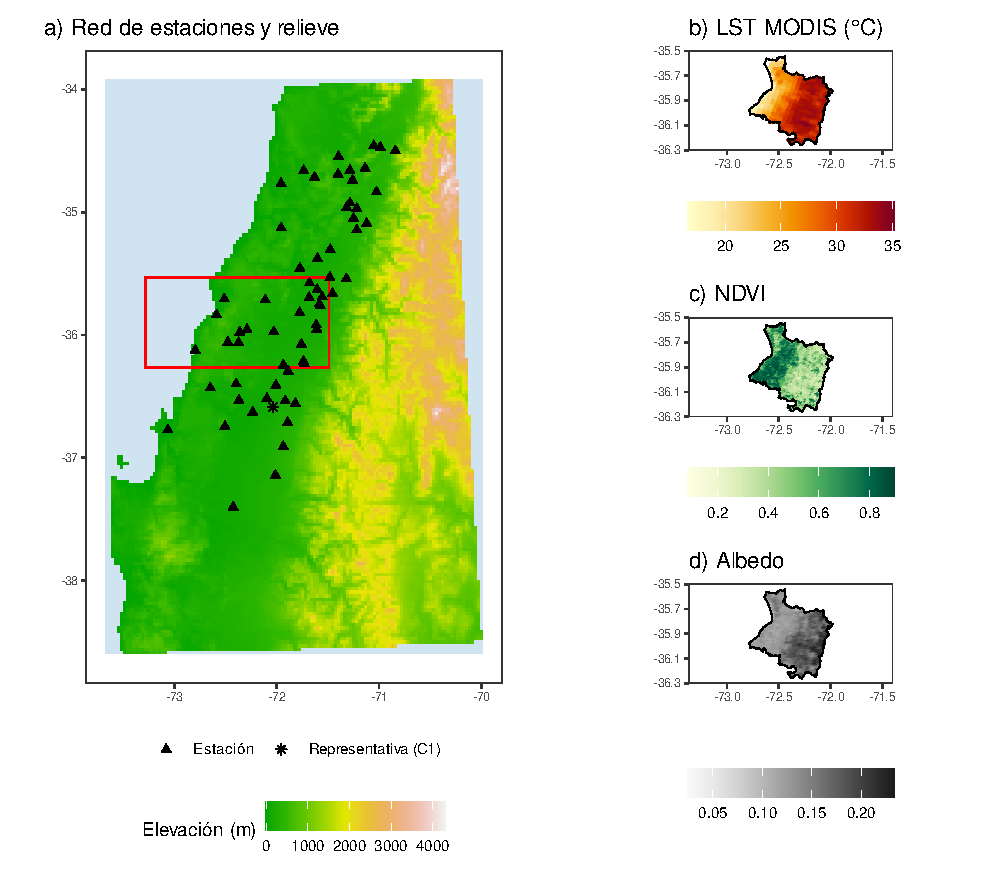
\includegraphics[width=\textwidth]{fig01_area.pdf}
\caption{(a) Red de estaciones meteorológicas sobre el relieve (Copernicus
GLO-90); el rectángulo rojo es la extensión de la escena y el asterisco la
estación representativa de C1. (b--d) Temperatura superficial, NDVI y albedo
MODIS del 15-02-2019 en la provincia de Cauquenes. Coordenadas geográficas
(WGS~84) solo para visualización.}\label{fig:area}
\end{figure}

\subsection{Observaciones satelitales}

Se usa la escena de ejemplo \code{cauquenes\_modis} de EarthFlux: el estado
de superficie MODIS colección~6.1 del 15 de febrero de 2019 (paso de Terra
cerca de las 14:08~UTC; nubosidad del mosaico h12v12 de 3~\%). Integra la
temperatura superficial diurna y las emisividades de las bandas 31--32 de
MOD11A1 \parencite{wan2021mod11a1,wan2014mod11c6}, el albedo de cielo blanco
de MCD43A3 \parencite{schaaf2021mcd43a3,schaaf2002brdf}, el NDVI de MOD13A2
\parencite{didan2021mod13a2} y el LAI de MCD15A2H
\parencite{myneni2021mcd15a2h}, en la grilla sinusoidal de
$\approx\SI{926,6}{\metre}$. La escena contiene \SceneCellsProvince
celdas dentro de la provincia, \SceneCellsValid
de ellas con todas las variables válidas. La procedencia de cada gránulo,
la máscara de calidad y las palabras de \emph{flags} se documentan en el
paquete. La elevación proviene del modelo Copernicus GLO-90, promediado a
cada celda.

\subsection{Observaciones meteorológicas}\label{sec:stations}

\StationDataText

Todas las estaciones se procesan con la tabla estándar y el control de
calidad de EarthFlux (\code{ef\_station\_table()}, \code{ef\_station\_qc()}),
que marca y nunca elimina en silencio. Las covariables de regionalización
son la elevación media de \SI{1}{\kilo\metre} (Copernicus GLO-90) y la
distancia a la costa (Natural Earth 1:10~m), en una grilla UTM~18S de
\SI{1}{\kilo\metre}. No se usan covariables derivadas de la superficie
(LST, NDVI) para evitar la circularidad entre la temperatura del aire
regionalizada y la temperatura superficial que gobierna la calibración de
$dT$ (decisión D-11).

\subsection{Referencias de validación}\label{sec:validation-data}

Se buscaron mediciones independientes de $\ETa$ o de flujo de calor latente
(covarianza de torbellinos, lisímetros) para la región y la fecha. La red
AmeriFlux registra cinco sitios en Chile, todos fuera del área (Chiloé,
Alerce Costero, Fray Jorge, Omora). Las torres de covarianza de torbellinos
operadas en viñedos y huertos de Talca y Ñuble
\parencite{carrascobenavides2014metric,ortegafarias2010twolayer} no tienen
datos públicos para febrero de 2019, y el único conjunto abierto cercano
encontrado (huertos de avellano en Ñuble, Zenodo) contiene salidas de un
modelo y no mediciones. Por lo tanto, \textbf{este estudio no dispone de
referencias independientes para validar la exactitud absoluta de $\ETa$}. La
validación se limita a las variables meteorológicas, para las que sí existen
observaciones independientes (validación cruzada espacial,
sección~\ref{sec:design}). Los reanálisis no se usan como verdad
observacional.

\section{Metodología}\label{sec:methods}

\subsection{Arquitectura de EarthFlux y niveles de evidencia}

EarthFlux (versión \EarthFluxVersion, commit \texttt{\EarthFluxCommit})
organiza la física de METRIC en funciones vectorizadas e independientes del
sensor (radiación, $G$, rugosidad, anclas, calibración de $H$, $LE$, $ET$),
un módulo de forzamiento meteorológico (tabla de estaciones, control de
calidad, ET de referencia FAO-56 y ASCE-EWRI) y un módulo de
regionalización con interfaz común para C1, C2 y C3 (\code{ef\_regionalize()},
\code{ef\_regionalize\_cv()}) y núcleo GWR propio verificado contra
\pkg{GWmodel} \parencite{gollini2015gwmodel}. Toda elección científica sin
fuente única carece de valor por defecto y queda registrada en la
procedencia; los valores físicamente anómalos se marcan con \emph{flags} y
no se truncan. El estudio se ejecuta exclusivamente con la API pública del
paquete, en un directorio separado de su código (\code{research/cedes2027/}).

Se distinguen cuatro niveles de evidencia (tabla~\ref{tab:verification}):
(1) \emph{verificación de ecuaciones}: contraste, término a término, de cada
formulación con su fuente primaria; (2) \emph{pruebas de software}:
pruebas unitarias, de invariantes y de integración ejecutadas en cada
\code{R CMD check}; (3) \emph{validación meteorológica}: error fuera de
muestra de las variables regionalizadas frente a estaciones no usadas en el
ajuste; y (4) \emph{validación de $\ETa$}: comparación con mediciones
independientes de flujos, no disponible en este estudio.

\subsection{Diseño experimental}\label{sec:design}

El estudio comprende tres experimentos (figura~\ref{fig:workflow}).

\begin{figure}[htbp]
\centering
\begin{tikzpicture}[node distance=4mm and 6mm, font=\footnotesize,
  box/.style={draw, rounded corners, align=center, fill=#1, minimum height=9mm, text width=3.1cm},
  box/.default=white, arr/.style={-{Stealth[length=2mm]}, thick}]
\node[box=gray!12] (st) {\NStations{} estaciones horarias\\(DMC, INIA, FDF, NOAA)};
\node[box=gray!12, below=of st] (dem) {Elevación y distancia\\a la costa (1 km)};
\node[box=gray!12, below=of dem] (modis) {Escena MODIS\\15-02-2019 (1 km)};
\node[box=teal!12, right=of st, yshift=-6.5mm] (reg) {Regionalización\\C1, C1-lap, C2-OLS,\\C2-IDW, C3-GWR};
\node[box=teal!12, right=of reg] (cv) {\textbf{Exp. R}: validación\\cruzada espacial\\anidada (90 días)};
\node[box=orange!15, below=of reg, yshift=-5mm] (metric) {METRIC: $R_n$, $G$, anclas,\\$r_{ah}$, $H$, $LE$, $\mathrm{ET_rF}$};
\node[box=orange!15, right=of metric] (m) {\textbf{Exp. M}: sustitución\\completa y de una\\variable por vez};
\node[box=orange!15, below=of m] (s) {\textbf{Exp. S}: Monte Carlo\\anclas, ruido MODIS,\\alternativas};
\node[box=gray!5, below=of metric] (eta) {$\mathrm{ET_a} = \mathrm{ET_rF}\cdot\mathrm{ET_r^{24}}$};
\draw[arr] (st) -- (reg); \draw[arr] (dem) -- (reg); \draw[arr] (reg) -- (cv);
\draw[arr] (reg) -- node[left, font=\scriptsize]{$T_a, e_a, u_2, \mathrm{ET_r}$} (metric);
\draw[arr] (modis) -- (metric); \draw[arr] (metric) -- (eta);
\draw[arr] (metric) -- (m); \draw[arr] (m) -- (s);
\end{tikzpicture}
\caption{Diseño del estudio. Los tres experimentos comparten estaciones,
covariables, escena, ecuaciones y criterios de calibración; solo cambia la
representación espacial del forzamiento meteorológico.}\label{fig:workflow}
\end{figure}


\paragraph{Experimento R: regionalización meteorológica.} Para cada hora
de paso (14:00~UTC) de los \NCVDays{} días entre el 1 de enero y el 31 de
marzo de 2019, y para la temperatura del aire, la presión de vapor y la
velocidad del viento a \SI{2}{\metre} (convertida desde la altura del
anemómetro con el perfil logarítmico de FAO-56), se evaluaron C1, C1-lap
(solo temperatura), C2-OLS, C2-IDW y C3-GWR mediante validación cruzada por
bloques espaciales de \SI{50}{\kilo\metre} (\NFolds{} pliegues). El ancho de
banda de GWR (núcleo bicuadrado, $k$ adaptativo, AICc) y la potencia de IDW
($p\in\{1,2,3\}$, LOOCV) se vuelven a seleccionar dentro de cada conjunto de
entrenamiento (validación anidada), de modo que ninguna estación de
evaluación interviene en la selección. La estación representativa de C1 se
eligió con una regla fijada antes de ver los errores (D-02): la estación
completa más cercana al centroide de la provincia. Las métricas son RMSE,
MAE, sesgo (predicho $-$ observado) y correlación de Pearson; sus intervalos
de confianza del 95~\% se obtuvieron por \emph{bootstrap} de bloques que
remuestrea días completos ($B=2000$), lo que conserva junta la dependencia
espacial de los errores de un mismo instante. La comparación con GWR se
hizo de forma pareada sobre las mismas predicciones fuera de muestra
(diferencia media de errores cuadráticos, $\Delta SE$).

\paragraph{Experimento M: propagación en METRIC.} Para el día de la escena
se regionalizaron las 24 horas locales (UTC$-3$) de las tres variables con
cada configuración, con las mismas estaciones, control de calidad,
covariables y horas; los vacíos horarios de hasta 6~h se rellenaron por
interpolación temporal y se contaron (D-09). Los campos se proyectaron a la
grilla MODIS. La $\ETr$ horaria de alfalfa (ASCE-EWRI) se calculó por píxel
a partir de los campos regionalizados y de la radiación de onda corta
modelada, igual para todas las configuraciones (D-04); $\ETr^{24}$ es la
suma de las 24 horas. METRIC se ejecutó con idénticas ecuaciones, máscaras,
insumos MODIS, criterios de anclas y condiciones de borde
(tabla~\ref{tab:options}). Las anclas se seleccionan solo con variables de
superficie (D-08) dentro de las celdas con todos los insumos válidos; si
el forzamiento es válido en toda la escena, las anclas son las mismas celdas
en todas las corridas (se verificó corrida por corrida), de modo que los
cambios de calibración se deben exclusivamente al forzamiento evaluado en
esas celdas. Se realizaron
dos tipos de corrida: (a) \emph{sustitución completa}, con cada
configuración; y (b) \emph{sustitución de una variable por vez}, partiendo de
C1 y reemplazando una sola entrada ($T_a$, $e_a$, $u_2$, $\ETr$ instantánea
o $\ETr^{24}$) por su campo C3-GWR. La comparación usa C1 como línea base
porque representa la práctica convencional, no porque se suponga correcta.


\begin{table}[htbp]
\centering\footnotesize
\caption{Opciones de METRIC comunes a todas las configuraciones (decisiones
del estudio; ver \texttt{docs/decisions.md}).}\label{tab:options}
\begin{tabularx}{\textwidth}{>{\raggedright\arraybackslash}p{4.3cm}>{\raggedright\arraybackslash}X>{\raggedright\arraybackslash}p{2.6cm}}
\toprule
Componente & Elección & Estado / decisión \\
\midrule
Onda corta incidente & Transmisividad particionada de Allen ($K_t = 1$), terreno plano & CANDIDATA \\
Flujo de calor del suelo & Bastiaanssen ($G/R_n$ en función de $T_s$, $\alpha$, NDVI) & VERIFICADA; D-05 \\
Rugosidad & $z_{om} = 0{,}018\,\mathrm{LAI}$, mínimo \SI{0,005}{\metre} & D-06 \\
Viento a la altura de mezcla & Perfil logarítmico desde \SI{2}{\metre}, $z_{om}$ de la estación \SI{0,015}{\metre}, $z_b = \SI{200}{\metre}$ & VERIFICADA \\
Estabilidad & Monin--Obukhov iterativa; $\psi_m$ estable a \SI{2}{\metre}; tolerancia 0,01; máx. 20 iteraciones & VERIFICADA; P0-10 \\
Anclas & Frías: NDVI $\ge P_{95}$ y 20\,\% más frío; calientes: NDVI $\le P_{10}$ y 20\,\% más cálido; mediana & CANDIDATA; D-08 \\
Condiciones de borde & $\mathrm{ET_rF}_{cold} = 1{,}05$; $LE_{hot} = 0$ & D-07 \\
Corrección de $T_s$ & $\Gamma = \SI{6,5}{\kelvin\per\kilo\metre}$ a la elevación mediana & VERIFICADA (forma) \\
Calor latente de vaporización & Constante, \SI{2,45}{\mega\joule\per\kilo\gram} & P0-7 \\
ET de referencia & Alfalfa, ASCE-EWRI horaria; $\mathrm{ET_r^{24}}$ = suma de 24 horas & VERIFICADA; D-04 \\
\bottomrule
\end{tabularx}
\end{table}

\paragraph{Experimento S: sensibilidad y robustez.} Con los forzamientos C1
y C3-GWR (o la mejor alternativa espacial factible) se realizaron
\NMC{} réplicas Monte Carlo de (S-A) los criterios de anclas y las
condiciones de borde (percentil de NDVI frío $\sim U(0{,}90;0{,}98)$, caliente
$\sim U(0{,}05;0{,}20)$, fracciones seleccionadas $\sim U(0{,}1;0{,}3)$,
$\ETrF_{cold}\sim U(1{,}00;1{,}10)$) y de (S-B) los insumos MODIS (LST con
ruido $N(0,\SI{1}{\kelvin})$ por píxel más un sesgo de escena
$N(0,\SI{0,5}{\kelvin})$, coherente con la exactitud de MOD11
\parencite{wan2014mod11c6}; albedo con error relativo $N(0;0{,}05)$), además
de (S-C) alternativas estructurales deterministas (G de Bastiaanssen frente
a Tasumi, piso de rugosidad, agregación de anclas). En S-A y S-B, la misma
perturbación se aplica a ambos forzamientos, lo que permite estimar el
efecto del forzamiento de forma pareada y compararlo con la dispersión
inducida por las otras fuentes. Con \NMC{} réplicas, el error estándar
Monte Carlo de una media es la desviación estándar dividida por
$\sqrt{\NMC}$, suficiente para las diferencias de interés.

\subsection{Reproducibilidad}

Los scripts del estudio (\code{research/cedes2027/scripts/}) descargan los
datos de fuentes públicas, registran sumas de verificación, fijan la
semilla (\num[group-separator={}]{\Seed}) y generan cada tabla, figura y
cifra del texto. Las cifras de este manuscrito se insertan desde un
archivo de macros generado a partir de las tablas de resultados, y cada una
está trazada a su archivo y procedimiento en el registro de afirmaciones
cuantitativas del material suplementario.

\section{Resultados}\label{sec:results}

\subsection{Verificación de componentes}\label{sec:res-verif}

La tabla~\ref{tab:verification} resume el estado de los componentes de la
cadena usada. De las \VerRows{} formulaciones del núcleo contrastadas por el
paquete con el manual de los autores del método \parencite{waters2002sebal},
\VerVerified{} están verificadas palabra por palabra, \VerCorroborated{}
corroboradas y \VerCandidate{} siguen como candidatas; el contraste detectó
\VerDiscrepancies{} discrepancias, \VerFixed{} de ellas corregidas en el
código. En este entorno de ejecución (R~4.3.3, \pkg{terra}~1.7-65) se
ejecutaron \NTests{} bloques de pruebas con \NExpectations{} expectativas:
\NTestsPassed{} bloques aprobados, \NTestsFailed{} fallos, \NTestsSkipped{}
omitidos por requerir dependencias opcionales y \NTestsError{} con error,
todos en la lectura de archivos HDF de MODIS por una incompatibilidad con
la versión local de \pkg{terra}; esa lectura no se usa en el estudio, que
parte de la escena ya preprocesada. Las pruebas de la cadena METRIC verifican
el cierre de energía en las anclas ($H = H_{target}$ con tolerancia relativa
$10^{-10}$), $LE = \Rnet - G - H$ en cada píxel y la reproducción de las
condiciones de borde de $\ETrF$; el núcleo GWR coincide con \pkg{GWmodel}
hasta $10^{-10}$. Dos componentes centrales de este estudio siguen como
candidatos: la transmisividad particionada de Allen y los criterios de
selección de anclas.

\begin{table}[htbp]
\centering\footnotesize
\caption{Componentes de la cadena METRIC usada, estado de verificación y
pruebas (fuente: \texttt{config/verification\_map.csv} y
\texttt{dev/VERIFICATION.md} del paquete).}\label{tab:verification}
\begin{tabularx}{\textwidth}{>{\raggedright\arraybackslash}p{3.4cm}>{\raggedright\arraybackslash}X>{\raggedright\arraybackslash}p{2.9cm}>{\raggedright\arraybackslash}p{3.1cm}r}
\toprule
Componente & Funciones & Estado & Fuente & Pruebas \\
\midrule
Radiación neta & \texttt{ef\_net\_radiation()} & VERIFICADA (SEBAL-Idaho 2002) & Waters et al. (2002), Ec. 2 & 63 \\
Onda corta incidente, terreno plano & \texttt{ef\_rs\_in(method = modelled)} & VERIFICADA (SEBAL-Idaho 2002) & Waters et al. (2002), Ec. 12 & 67 \\
Transmisividad particionada (Allen) & \texttt{ef\_tau\_sw(method = allen)} & CANDIDATA & ASCE-EWRI (2005), forma de Allen (1996) & 67 \\
Emisividad atmosférica & \texttt{ef\_atm\_emissivity()} & VERIFICADA (SEBAL-Idaho 2002) & Waters et al. (2002), Ec. 22 & 67 \\
Onda larga incidente y emitida & \texttt{ef\_rl\_in(), ef\_rl\_out()} & VERIFICADA (SEBAL-Idaho 2002) & Waters et al. (2002), Ecs. 20-23 & 67 \\
Flujo de calor del suelo (Bastiaanssen) & \texttt{ef\_g(method = bastiaanssen)} & VERIFICADA (SEBAL-Idaho 2002) & Waters et al. (2002), Ec. 24 & 39 \\
Flujo de calor del suelo (Tasumi) & \texttt{ef\_g(method = tasumi)} & CANDIDATA & Tasumi (2003) & 39 \\
Rugosidad por LAI & \texttt{ef\_zom(method = lai)} & VERIFICADA (SEBAL-Idaho 2002) & Waters et al. (2002), Ec. 31a & 15 \\
Viento a altura de mezcla y u* & \texttt{ef\_blending\_wind(), ef\_ustar()} & VERIFICADA (SEBAL-Idaho 2002) & Waters et al. (2002), Ecs. 27, 29, 30 & 15 \\
Resistencia aerodinámica y estabilidad & \texttt{ef\_rah(), psi\_m, psi\_h, L} & VERIFICADA (SEBAL-Idaho 2002) & Waters et al. (2002), Ecs. 26, 34-41 & 39 \\
Calibración dT y calor sensible & \texttt{ef\_calibrate\_h(), ef\_dt\_coef(), ef\_sensible\_heat()} & VERIFICADA (forma); procedimiento P0-10 & Waters et al. (2002), Ecs. 25, 32, 33 & 30 \\
Condiciones de borde de las anclas & \texttt{ef\_anchor\_conditions()} & VERIFICADA (forma) & Waters et al. (2002), p. 30-31 & 9 \\
Criterios de selección de anclas & \texttt{ef\_select\_anchors(), ef\_anchor\_criteria()} & CANDIDATA & Waters et al. (2002), ap. 7 & 28 \\
Calor latente, ET instantánea, ETrF y ETa diaria & \texttt{ef\_latent\_heat(), ef\_et\_inst(), ef\_etrf(), ef\_et\_daily()} & VERIFICADA (FAO-56; SEBAL-Idaho 2002) & Waters et al. (2002), Ecs. 1, 42-44 & 44 \\
ET de referencia ASCE-EWRI horaria & \texttt{ef\_ref\_et(), ef\_ref\_net\_radiation(), ef\_ref\_soil\_heat\_flux()} & VERIFICADA (ecuaciones y constantes) & ASCE-EWRI (2005) & 58 \\
Regionalización C1/C2/C3 y núcleo GWR & \texttt{ef\_regionalize(), ef\_regionalize\_cv(), ef\_gwr\_*()} & CANDIDATA (corroborada con GWmodel a 1e-10) & Brunsdon et al. (1996); Gollini et al. (2015) & 75 \\
\bottomrule
\end{tabularx}

\end{table}

\subsection{Regionalización meteorológica}\label{sec:res-reg}

La regla D-02 seleccionó como estación representativa
\emph{\RepStationName}, a \RepStationDist{}~km del centroide de la provincia: la estación más
cercana con registros completos de temperatura, humedad y viento. La validación
cruzada espacial (\NFolds{} pliegues, \NCVDays{} días, \num[round-precision=0]{\NCVPred}
predicciones fuera de muestra) entregó los errores de la tabla~\ref{tab:cv}
y la figura~\ref{fig:cv}.

Para la temperatura del aire, todas las alternativas espaciales superaron a
la estación representativa (RMSE C1 = \CVTaCOneRmse{}~\si{\celsius},
IC~95\,\% [\CVTaCOneRmseLo; \CVTaCOneRmseHi]). La corrección por gradiente
vertical no mejoró a C1 (C1-lap: \CVTaCOneLapRmse{}~\si{\celsius}), lo que
indica que la diferencia entre la estación y el resto del territorio no es
principalmente altitudinal. GWR (\CVTaCThreeGWRRmse{}~\si{\celsius}
[\CVTaCThreeGWRRmseLo; \CVTaCThreeGWRRmseHi]) superó a C1 y a la regresión
global (\CVTaCTwoOLSRmse{}~\si{\celsius}); en la comparación pareada, su error
cuadrático fue menor que el de C1 en \PairTaCOneDse{}~\si{\celsius\squared}
en promedio (IC [\PairTaCOneLo; \PairTaCOneHi]) y que el de C2-OLS en
\PairTaCTwoOLSDse{}~\si{\celsius\squared} ([\PairTaCTwoOLSLo; \PairTaCTwoOLSHi]).
Sin embargo, el método de menor error fue IDW (\CVTaCTwoIDWRmse{}~\si{\celsius}
[\CVTaCTwoIDWRmseLo; \CVTaCTwoIDWRmseHi]): la diferencia pareada GWR$-$IDW fue
positiva, \PairTaCTwoIDWDse{}~\si{\celsius\squared} (IC
[\PairTaCTwoIDWLo; \PairTaCTwoIDWHi]), y GWR tuvo menor error absoluto que IDW
solo en el \PairTaCTwoIDWShare\,\% de las predicciones. El patrón se repite
para la presión de vapor: IDW (\CVEaCTwoIDWRmse{}~kPa) $<$ GWR
(\CVEaCThreeGWRRmse{}~kPa) $<$ OLS (\CVEaCTwoOLSRmse{}~kPa) $<$ C1
(\CVEaCOneRmse{}~kPa), con la diferencia GWR$-$IDW también positiva
([\PairEaCTwoIDWLo; \PairEaCTwoIDWHi]~\si{\kilo\pascal\squared}). Los sesgos
medios fueron pequeños para todos los métodos espaciales ($|$sesgo$|$ $\le$
\num{0.05}~\si{\celsius}).

Los residuos de C1 y de la regresión global conservaron dependencia
espacial (I de Moran mediano \MoranTaCOneI{} y \MoranTaCTwoOLSI{} para la
temperatura, significativo en el \MoranTaCOneSig\,\% y \MoranTaCTwoOLSSig\,\%
de los instantes), mientras que IDW y GWR la eliminaron casi por completo
(\MoranTaCTwoIDWSig\,\% y \MoranTaCThreeGWRSig\,\% de instantes
significativos). La densidad de la red condicionó a GWR más que a IDW
(figura~\ref{fig:density}): con \DensTaCThreeGWRQuarterN{} estaciones (25\,\%)
el RMSE de la temperatura fue \DensTaCThreeGWRQuarter{}~\si{\celsius} con GWR y
\DensTaCTwoIDWQuarter{}~\si{\celsius} con IDW, frente a \DensTaCThreeGWRAll{} y
\DensTaCTwoIDWAll{}~\si{\celsius} con la red completa.

El viento solo se mide en \NStationsWind{} estaciones. Con ellas, GWR no pudo
ajustarse en ninguno de los \CVWindCThreeGWRTotal{} casos de validación
(sin ancho de banda factible), y la regresión global produjo predicciones
fuera del dominio físico (máximo \CVWindOLSMax{}~\si{\metre\per\second};
\CVWindOLSNeg{} predicciones negativas) con RMSE de
\CVWindCTwoOLSRmse{}~\si{\metre\per\second}, frente a \CVWindCOneRmse{} de C1
y \CVWindCTwoIDWRmse{}~\si{\metre\per\second} de IDW.

\begin{figure}[htbp]
\centering
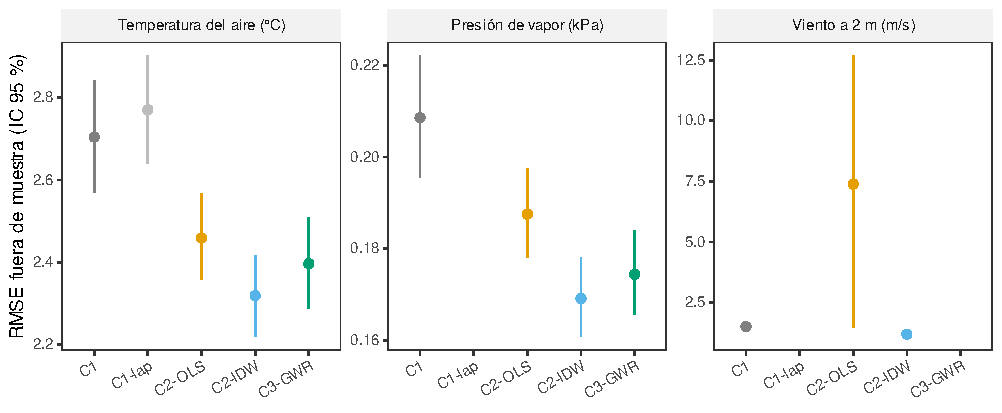
\includegraphics[width=\textwidth]{fig03_cv_rmse.pdf}
\caption{RMSE fuera de muestra (validación cruzada espacial anidada) por
variable y configuración, con IC~95\,\% por \emph{bootstrap} de días. GWR del
viento no fue factible (sin punto).}\label{fig:cv}
\end{figure}

\begin{table}[htbp]
\centering
\footnotesize
\caption{Validación cruzada espacial anidada de la regionalización a la hora del paso (14:00 UTC, enero--marzo de 2019).}\label{tab:cv}
\begin{threeparttable}
\begin{tabular}{llrlrlrr}
\toprule
Variable & Config. & $n$ & RMSE [IC 95\,\%] & MAE & Sesgo [IC 95\,\%] & $r$ & Fallidas \\
\midrule
$T_a$ (\si{\celsius}) & C1 & 5498 & 2,70 [2,57; 2,84] & 2,10 & -0,16 [-0,38; 0,07] & 0,70 & 0 \\
 & C1-lap & 5498 & 2,77 [2,64; 2,90] & 2,17 & -0,05 [-0,27; 0,18] & 0,68 & 0 \\
 & C2-OLS & 5588 & 2,46 [2,36; 2,57] & 1,92 & -0,01 [-0,02; 0,00] & 0,75 & 0 \\
 & C2-IDW & 5588 & 2,32 [2,22; 2,42] & 1,83 & 0,01 [-0,01; 0,03] & 0,78 & 0 \\
 & C3-GWR & 5588 & 2,40 [2,29; 2,51] & 1,85 & -0,04 [-0,07; -0,02] & 0,76 & 0 \\
$e_a$ (\si{\kilo\pascal}) & C1 & 5495 & 0,209 [0,195; 0,222] & 0,153 & -0,024 [-0,043; -0,005] & 0,69 & 0 \\
 & C2-OLS & 5585 & 0,188 [0,178; 0,198] & 0,135 & 0,003 [0,002; 0,004] & 0,73 & 0 \\
 & C2-IDW & 5585 & 0,169 [0,161; 0,178] & 0,120 & -0,005 [-0,006; -0,003] & 0,79 & 0 \\
 & C3-GWR & 5585 & 0,174 [0,166; 0,184] & 0,122 & -0,002 [-0,004; 0,000] & 0,77 & 0 \\
$u_2$ (\si{\metre\per\second}) & C1 & 505 & 1,51 [1,37; 1,64] & 1,20 & 0,63 [0,46; 0,80] & 0,52 & 0 \\
 & C2-OLS & 595 & 7,39 [1,48; 12,69] & 1,57 & 0,10 [-0,22; 0,70] & 0,08 & 0 \\
 & C2-IDW & 595 & 1,19 [1,10; 1,29] & 0,91 & -0,04 [-0,06; -0,02] & 0,58 & 0 \\
 & C3-GWR & 0 & \multicolumn{4}{l}{no factible (sin ancho de banda factible)} & 595 \\
\bottomrule
\end{tabular}
\begin{tablenotes}\footnotesize
\item $n$: predicciones fuera de muestra. Sesgo = predicho $-$ observado. IC: \emph{bootstrap} de días completos ($B = 2000$).
\item C1 no se evalúa en su propia estación. Fallidas: predicciones cuyo pliegue no pudo ajustarse con las estaciones de entrenamiento (p.\,ej., GWR o regresión global con menos estaciones que parámetros + 3).
\end{tablenotes}
\end{threeparttable}
\end{table}


\begin{figure}[htbp]
\centering
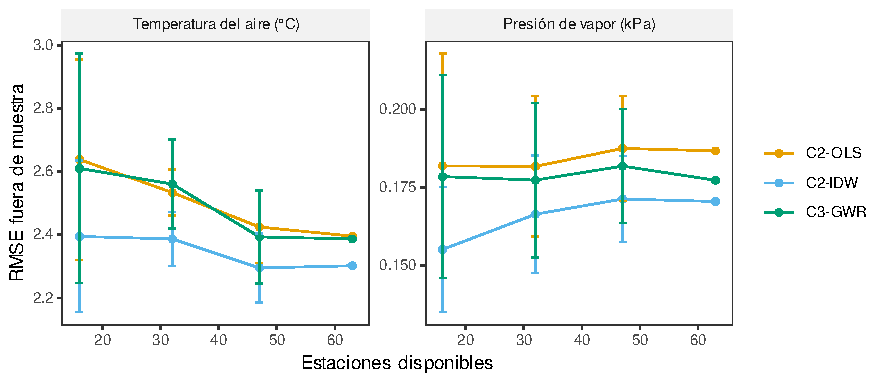
\includegraphics[width=0.85\textwidth]{fig09_density.pdf}
\caption{RMSE de validación cruzada según la fracción de estaciones
disponible (media de 10 subconjuntos aleatorios en 30 días; la barra indica
$\pm 1$ desviación estándar).}\label{fig:density}
\end{figure}

\subsection{Campos meteorológicos y balance de energía superficial}\label{sec:res-eb}

A la hora del paso, la escena recibió de C1 un valor único de temperatura
(\MFTaCOneMean~\si{\celsius}), presión de vapor (\MFEaCOneMean~kPa) y viento
(\MFWindCOneMean~\si{\metre\per\second}). Las configuraciones espaciales
produjeron campos con medias y amplitudes distintas
(figura~\ref{fig:forcing}): la temperatura media fue \MFTaCTwoIDWMean~\si{\celsius}
(DE espacial \MFTaCTwoIDWSd) con IDW y \MFTaCThreeGWRMean~\si{\celsius}
(DE \MFTaCThreeGWRSd) con GWR. El campo de GWR presentó máximos locales de
hasta \RangeTaCThreeGWRMax~\si{\celsius} en la Cordillera de la Costa, por
encima del máximo observado en las estaciones a esa hora
(\RangeTaCThreeGWRObsMax~\si{\celsius}) en el \RangeTaCThreeGWRAbove\,\% de
las celdas procesadas: los coeficientes locales se extrapolan en terreno sin
estaciones, un problema que la validación cruzada en las estaciones no puede
detectar. Ninguna otra configuración salió del rango observado. La $\ETr^{24}$
media de la escena fue \MFEtrDayCOneMean~mm/d con C1, \MFEtrDayCThreeGWRMean~mm/d
con GWR, \MFEtrDayCTwoIDWMean~mm/d con IDW y \MFEtrDayCTwoOLSMean~mm/d con la
regresión global. Estos resultados confirman H1: las configuraciones
producen diferencias espaciales identificables en las variables que entran
en METRIC (salvo el viento de GWR, que no fue factible).

\begin{figure}[htbp]
\centering
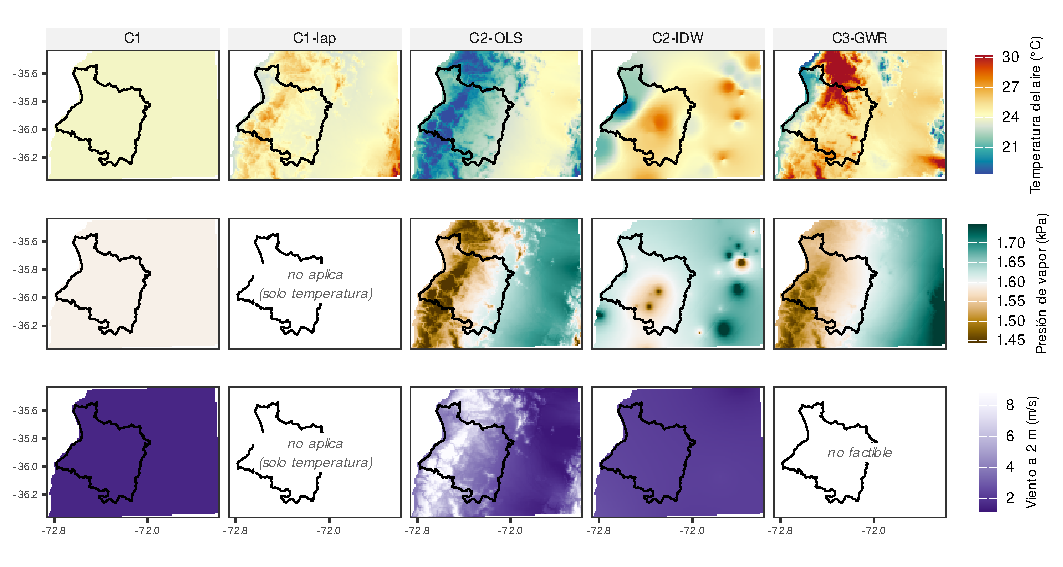
\includegraphics[width=\textwidth]{fig04_forcing_maps.pdf}
\caption{Temperatura del aire, presión de vapor y viento a 2~m regionalizados
a las 14:00~UTC del 15-02-2019 por configuración (grilla UTM~18S de 1~km;
mostrados en coordenadas geográficas). El viento de C3-GWR se reemplazó por
el de C1 (D-14).}\label{fig:forcing}
\end{figure}

Las celdas ancla fueron idénticas en \NRunsSameAnchors{} de las \NRuns{}
corridas; la excepción es C2-OLS, cuyo dominio válido se redujo a
\num[round-precision=0]{\OLSValidCells} celdas porque el viento regionalizado
salió del dominio físico, de modo que sus anclas se seleccionaron dentro de
ese dominio y C2-OLS no es comparable con el resto. Los cambios del forzamiento se tradujeron en cambios de la
calibración: $b$ varió entre \CalCThreeGWRB{} (GWR) y \CalCTwoIDWB{} (IDW) y
$a$ entre \CalCThreeGWRA{} y \CalCTwoIDWA~K (tabla~\ref{tab:metric}). La
radiación neta media aumentó \DRnCThreeGWRMean~\si{\watt\per\square\metre}
con GWR respecto de C1 (\MRnCOneMean{} frente a \MRnCThreeGWRMean~\si{\watt\per\square\metre})
y el calor sensible \DHCThreeGWRMean~\si{\watt\per\square\metre} (P5--P95:
\DHCThreeGWRLo{} a \DHCThreeGWRHi), de modo que el calor latente instantáneo
casi no cambió (\MLECOneMean{} frente a \MLECThreeGWRMean~\si{\watt\per\square\metre})
y la fracción $\ETrF$ media tampoco (\MEtrfCOneMean{} frente a
\MEtrfCThreeGWRMean; diferencia \DEtrfCThreeGWRPct\,\%). Con IDW, cuyo campo
de viento difiere del de C1, $\ETrF$ disminuyó \DEtrfCTwoIDWPct\,\%. La
figura~\ref{fig:eb} muestra los cuatro flujos por configuración.

\begin{table}[htbp]
\centering
\footnotesize
\caption{Balance de energía y $\mathrm{ET_a}$ de la escena de Cauquenes (15-02-2019) por configuración: media (desviación estándar espacial) y parámetros de calibración.}\label{tab:metric}
\begin{threeparttable}
\begin{tabular}{lrrrrr}
\toprule
Variable & C1 & C1-lap & C2-OLS & C2-IDW & C3-GWR \\
\midrule
$R_n$ & 475 (55) & 477 (56) & 449 (62) & 478 (49) & 483 (54) \\
$G$ & 58 (15) & 59 (15) & 66 (10) & 59 (16) & 59 (15) \\
$H$ & 267 (73) & 266 (74) & 325 (31) & 278 (79) & 271 (72) \\
$LE$ & 149 (135) & 153 (137) & 58 (87) & 140 (133) & 152 (132) \\
$\mathrm{ET_rF}$ & 0,40 (0,36) & 0,40 (0,37) & 0,15 (0,23) & 0,37 (0,38) & 0,40 (0,37) \\
$\mathrm{ET_a}$ (mm/d) & 3,45 (3,12) & 3,54 (3,17) & 1,04 (1,51) & 2,48 (2,26) & 2,76 (2,25) \\
$\mathrm{ET_r^{24}}$ (mm/d) & 8,56 (0,01) & 8,72 (0,26) & 6,95 (0,30) & 7,38 (0,86) & 7,56 (0,85) \\
\midrule
$a$ (K) & -65,73 & -67,00 & -30,77 & -73,83 & -64,94 \\
$b$ (--) & 0,231 & 0,236 & 0,115 & 0,258 & 0,229 \\
Iteraciones & 9 & 9 & 6 & 7 & 9 \\
$\mathrm{ET_r}$ inst. ancla fría (mm/h) & 0,544 & 0,554 & 0,563 & 0,535 & 0,535 \\
$u_{200}$ ancla fría (m/s) & 2,99 & 2,99 & 8,69 & 4,65 & 2,99 \\
Celdas con $\mathrm{ET_a} < 0$ & 77 & 74 & 156 & 102 & 58 \\
\bottomrule
\end{tabular}
\begin{tablenotes}\footnotesize
\item Flujos en \si{\watt\per\square\metre}. Las celdas ancla son las mismas en todas las configuraciones.
\end{tablenotes}
\end{threeparttable}
\end{table}


\begin{figure}[htbp]
\centering
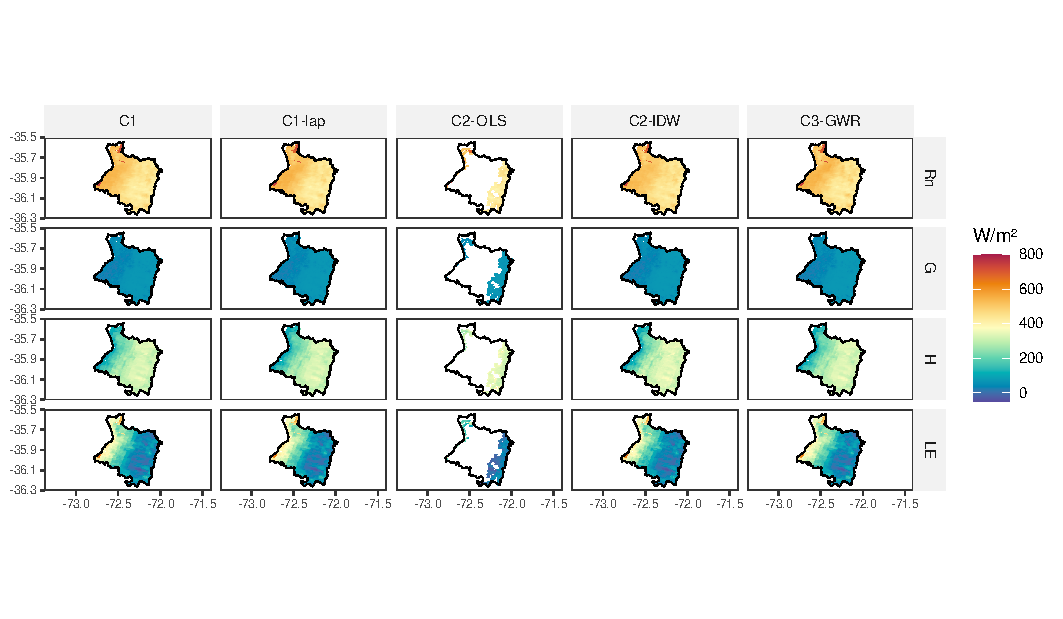
\includegraphics[width=\textwidth]{fig05_energy_balance.pdf}
\caption{Radiación neta, flujo de calor del suelo, calor sensible y calor
latente instantáneos (\si{\watt\per\square\metre}) por configuración.
C2-OLS tiene celdas sin datos donde el viento regionalizado salió del
dominio físico.}\label{fig:eb}
\end{figure}

\subsection{Evapotranspiración real}\label{sec:res-eta}

La $\ETa$ media de la escena fue \MEtaCOneMean~mm/d con C1,
\MEtaCOneLapMean~mm/d con C1-lap, \MEtaCTwoIDWMean~mm/d con IDW,
\MEtaCThreeGWRMean~mm/d con GWR y \MEtaCTwoOLSMean~mm/d con la regresión
global, esta última sobre solo \num[round-precision=0]{\OLSValidCells} celdas
válidas (figura~\ref{fig:eta}). Frente a C1, GWR redujo la $\ETa$ media en
\DEtaCThreeGWRMean~mm/d (\DEtaCThreeGWRPct\,\%), con diferencias locales
entre \DEtaCThreeGWRLo{} y \DEtaCThreeGWRHi~mm/d (P5--P95) y
$|\Delta\ETa| > 0{,}5$~mm/d en el \DEtaCThreeGWRShare\,\% de las celdas; IDW la
redujo en \DEtaCTwoIDWMean~mm/d (\DEtaCTwoIDWPct\,\%). La correlación espacial
entre los mapas fue alta (el patrón relativo se conserva), por lo que las
configuraciones cambian sobre todo el nivel y la amplitud de $\ETa$, no su
estructura.

La sustitución de una variable por vez (figura~\ref{fig:attr}) muestra que
el efecto no es uniforme entre vías de entrada (H2). La $\ETr^{24}$
regionalizada explicó casi todo el cambio: por sí sola modificó la $\ETa$
en \DEtaOatEtrDayMean~mm/d (\DEtaOatEtrDayPct\,\%). La $\ETr$ instantánea,
que actúa a través de la condición del ancla fría, cambió la calibración
($a$ = \CalOatEtrInstA~K; $b$ = \CalOatEtrInstB) con un efecto medio de
\DEtaOatEtrInstMean~mm/d y compensaciones locales (P5--P95:
\DEtaOatEtrInstLo{} a \DEtaOatEtrInstHi~mm/d). La temperatura del aire
contribuyó \DEtaOatTaMean~mm/d, la presión de vapor \DEtaOatEaMean~mm/d y el
viento (campo IDW, D-16) \DEtaOatWindMean~mm/d. Sin el viento, que en la
corrida conjunta de GWR es el de C1, la suma de los efectos individuales
($T_a$, $e_a$, $\ETr$ instantánea y $\ETr^{24}$) es prácticamente igual al
efecto conjunto (\DEtaCThreeGWRMean~mm/d): en esta escena, los efectos son
aproximadamente aditivos. En síntesis, la calibración interna absorbió casi
por completo el efecto del forzamiento sobre el balance instantáneo, y la
diferencia de $\ETa$ entró por la extrapolación diaria.

\begin{figure}[htbp]
\centering
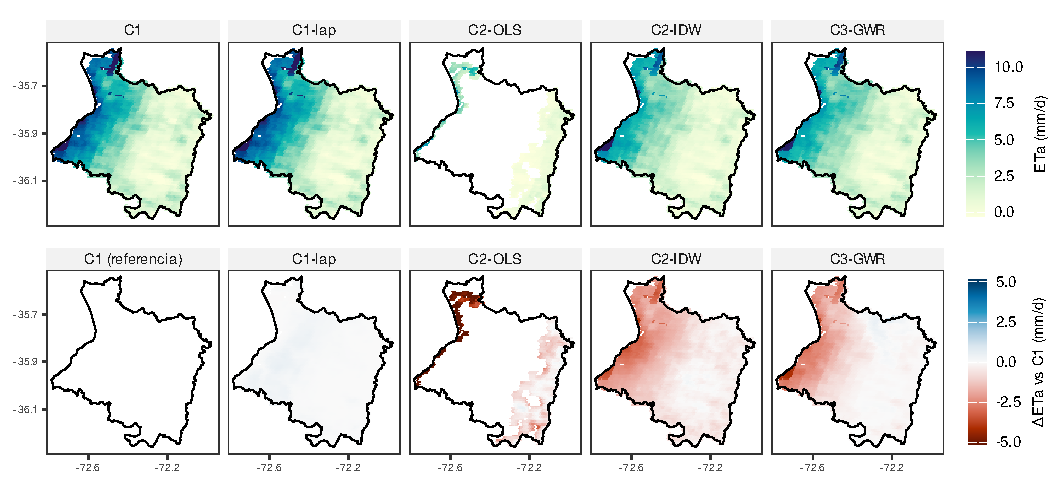
\includegraphics[width=\textwidth]{fig06_eta_maps.pdf}
\caption{Arriba: $\ETa$ diaria (mm/d) por configuración. Abajo: diferencia
respecto de C1 (mm/d). Escala común; valores fuera del rango P1--P99
saturados.}\label{fig:eta}
\end{figure}

\begin{figure}[htbp]
\centering
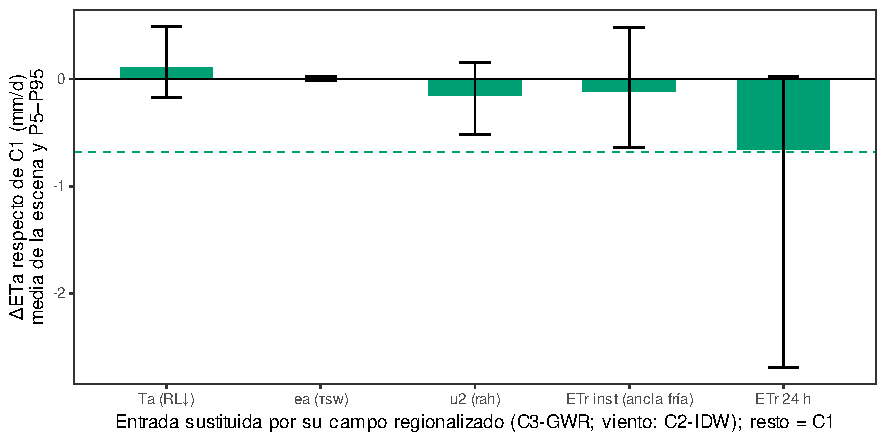
\includegraphics[width=0.8\textwidth]{fig07_attribution.pdf}
\caption{Cambio de la $\ETa$ media de la escena al reemplazar una sola
entrada de C1 por su campo regionalizado (C3-GWR; viento: C2-IDW). Barras de
error: P5--P95 de las diferencias por celda. Línea discontinua: sustitución
completa por C3-GWR.}\label{fig:attr}
\end{figure}

\subsection{Validación independiente}\label{sec:res-val}

No se dispuso de mediciones independientes de $\ETa$ o de flujo de calor
latente para el área y la fecha (sección~\ref{sec:validation-data}). Por lo
tanto, no se calcularon métricas de exactitud de $\ETa$ y \textbf{ninguna de
las diferencias anteriores puede interpretarse como mejora o deterioro de la
exactitud}. La única validación independiente del estudio es la de las
variables meteorológicas (sección~\ref{sec:res-reg}), evaluada fuera de
muestra en \NCVDays{} días.

\subsection{Sensibilidad y robustez}\label{sec:res-sens}

Las \NMC{} réplicas de criterios de anclas y condiciones de borde (S-A)
produjeron una dispersión de la $\ETa$ media de la escena de
\SACOneSd~mm/d (DE) con el forzamiento C1 y \SACThreeGWRSd~mm/d con GWR; el
ruido de los insumos MODIS (S-B) produjo \SBCOneSd{} y \SBCThreeGWRSd~mm/d,
respectivamente (figura~\ref{fig:sens}). En cada réplica, la diferencia
pareada GWR$-$C1 se mantuvo: \SAEffMean~mm/d (P2,5--P97,5:
\SAEffLo{} a \SAEffHi) bajo S-A y \SBEffMean~mm/d (\SBEffLo{} a \SBEffHi) bajo
S-B, con el mismo signo en el \SAEffSign\,\% y \SBEffSign\,\% de las réplicas.
Las alternativas estructurales (S-C) modificaron la $\ETa$ media de C1 de
\SCBaseCOne{} a \SCgTasumiCOne~mm/d (G de Tasumi), \SCZomFloorCOne~mm/d (piso
de rugosidad de 0,01~m) y \SCAggregateMeanCOne~mm/d (anclas por media). El ruido de LST desplazó hacia arriba la $\ETa$ media de C1
(intervalo \SBCOneLo--\SBCOneHi~mm/d frente a \SCBaseCOne~mm/d sin ruido), porque
la selección de anclas por extremos de LST es sensible al ruido por píxel. Todas
las calibraciones convergieron (\SACOneConv\,\% y \SBCOneConv\,\% de las
réplicas).

\begin{figure}[htbp]
\centering
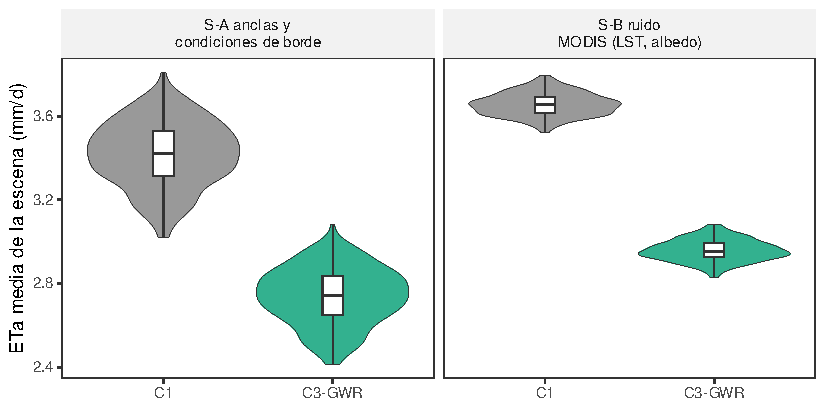
\includegraphics[width=0.85\textwidth]{fig08_sensitivity.pdf}
\caption{Distribución de la $\ETa$ media de la escena en \NMC{} réplicas
Monte Carlo de los criterios de anclas y condiciones de borde (S-A) y del
ruido de los insumos MODIS (S-B), con los forzamientos C1 y
C3-GWR.}\label{fig:sens}
\end{figure}

\section{Discusión}\label{sec:discussion}

\subsection{¿Regionaliza mejor GWR?}

En la red pública de la región del Maule, GWR mejoró de forma significativa
a la estación representativa y a la regresión global para la temperatura y
la presión de vapor, pero no superó a IDW, el interpolador más simple. Este
resultado es coherente con revisiones que muestran que la ventaja de los
métodos con covariables depende de que la relación con ellas sea fuerte y
estable frente a la densidad de observaciones \parencite{li2014interpolation}.
En este caso, la corrección por gradiente vertical no mejoró a C1, lo que
indica que, a la hora del paso (10:00 hora local), la variación de la
temperatura entre la costa, el secano y el valle no se explica
principalmente por la elevación, sino por la influencia marina y la
estructura de la capa límite, que la distancia a la costa solo captura de
forma parcial. GWR, además, necesita más estaciones que IDW para alcanzar su
rendimiento (figura~\ref{fig:density}) y, entre estaciones, puede producir
campos fuera del rango observado por extrapolación local de los
coeficientes \parencite{wheeler2005multicollinearity}; aquí afectó al
\RangeTaCThreeGWRAbove\,\% de las celdas procesadas. Estas dos limitaciones
no aparecen en las métricas de validación cruzada, que solo evalúan en las
estaciones, y son relevantes para cualquier aplicación que use GWR como
forzamiento de un modelo físico. Para el viento, medido en solo
\NStationsWind{} estaciones, ni GWR ni la regresión global son utilizables;
la regresión global extrapoló valores físicamente imposibles, que
EarthFlux conservó y marcó en vez de truncarlos. En conjunto, H3 y H4 se
confirman: la utilidad de GWR depende de la red y de la variable, y la mayor
complejidad no garantizó mayor exactitud.

\subsection{¿Cambia la $\ETa$?}

Sí, y de forma sustancial: con el mismo estado de superficie, las mismas
anclas y las mismas ecuaciones, la $\ETa$ media de la escena varió entre
\MEtaCTwoIDWMean{} y \MEtaCOneLapMean~mm/d entre las configuraciones con
cobertura completa. El experimento de sustitución explica el mecanismo. La calibración
interna de METRIC absorbió casi por completo los cambios del forzamiento
instantáneo: el ajuste de $a$ y $b$ en las anclas compensó el cambio de
$R_{L\downarrow}$ y del viento, y la fracción $\ETrF$ con GWR quedó a menos de
1\,\% de la de C1. Esta es la propiedad buscada por el diseño de METRIC
\parencite{allen2007metric1}, y aquí se cuantifica de forma explícita. La
diferencia de $\ETa$ entró por la extrapolación diaria $\ETa = \ETrF\cdot\ETr^{24}$:
la $\ETr^{24}$ de la estación representativa, ubicada en el valle central a
\RepStationDist~km, es mayor que la que los métodos espaciales asignan al
secano y a la costa (\MFEtrDayCOneMean{} frente a \MFEtrDayCThreeGWRMean~mm/d
con GWR). Esto confirma H2: la
propagación no es uniforme entre vías de entrada, y la vía dominante es la
menos discutida en la literatura sobre selección de anclas
\parencite{long2013endmember,bhattarai2017endmember}. Una consecuencia
práctica es que, en territorios con gradiente costa--interior, la
representatividad de la $\ETr^{24}$ puede pesar más que el refinamiento de
la calibración.

El efecto del forzamiento fue robusto frente a las otras fuentes de
incertidumbre evaluadas. La diferencia pareada GWR$-$C1 (\SAEffMean~mm/d)
mantuvo su signo en todas las réplicas y fue \RatioSA{} veces mayor que la
dispersión inducida por los criterios de anclas y las condiciones de borde
(DE \SACOneSd~mm/d) y \RatioSB{} veces mayor que la inducida por el ruido de
LST y albedo (DE \SBCOneSd~mm/d). Entre las alternativas estructurales, la
agregación de las anclas por media en lugar de mediana tuvo un efecto mayor
que la dispersión de los criterios (\SCAggregateMeanCOne{} frente a
\SCBaseCOne~mm/d), lo que recuerda la fragilidad de la calibración a 1~km
\parencite{tang2013scale,long2011sebalsensitivity}.

\subsection{Cambio entre modelos no es mejora de exactitud}

Ninguna de las diferencias de $\ETa$ puede calificarse como mejora o
deterioro, porque no existen mediciones independientes de flujos para la
escena. Sí puede afirmarse algo más débil pero útil: la elección del
forzamiento introduce en la $\ETa$ una incertidumbre del orden de
\DEtaCThreeGWRPct{} a \DEtaCTwoIDWPct\,\% de la media de la escena, mayor que
la debida a los insumos satelitales y a la calibración evaluadas aquí, y esa
incertidumbre debería reportarse junto con cualquier mapa de $\ETa$. Si la
$\ETr^{24}$ espacial es más representativa del secano que la de una estación
de valle ---lo que la validación meteorológica sugiere para sus insumos,
temperatura y humedad---, la $\ETa$ convencional estaría sobrestimada en esta
escena. Esa hipótesis queda planteada para ser contrastada con mediciones,
no demostrada.

\subsection{Contribución de EarthFlux y comparación con antecedentes}

Las ecuaciones de METRIC, FAO-56, ASCE-EWRI y GWR no son nuevas. La
contribución de EarthFlux está en la implementación y en lo que hace
posible: (i) física independiente del sensor con verificación documentada
contra fuente primaria; (ii) forzamiento intercambiable bajo una interfaz
común, que permitió comparar cinco configuraciones cambiando un argumento;
(iii) validación cruzada espacial anidada sin filtración; (iv) diagnósticos
que conservaron y marcaron valores fuera de dominio, como las predicciones
de viento de la regresión global; y (v) reproducibilidad completa de cada
cifra. Frente a \pkg{water} \parencite{olmedo2016water}, que implementa METRIC
para Landsat con una estación, EarthFlux agrega el forzamiento espacial y su
evaluación. El propio estudio detectó un error en el script de análisis
---covariables extraídas de una grilla que no cubría todas las estaciones---,
gracias a que el paquete registra las estaciones excluidas y su motivo, en
lugar de excluirlas en silencio.

\subsection{Implicaciones para la gestión sostenible del agua}

En volumen, el desacuerdo entre GWR y la estación representativa equivale a
\VolDiffAbsCThreeGWR{} millones de m³ en un solo día de verano sobre la provincia
(un caudal medio de unos \VolDiffFlowCThreeGWR~m³/s). Esto plantea una pregunta de
valor de la información: antes de invertir en mapas de $\ETa$ más finos o en más
estaciones, conviene saber cuánto cambia la estimación y por qué vía; aquí,
casi todo el cambio entra por la $\ETr$ diaria. Para la gestión del uso consuntivo, la valoración del agua y la evaluación
de programas de riego, el resultado más relevante es que la elección del
forzamiento meteorológico cambia la $\ETa$ estimada en una magnitud similar
a la de las decisiones que esos instrumentos buscan informar. En términos
prácticos: (a) los mapas de $\ETa$ usados en fiscalización o contabilidad
hídrica deberían declarar su forzamiento y acompañarse de un análisis de
sensibilidad a esa elección; (b) en el secano costero e interior de Chile
central, la densificación de estaciones con viento y radiación ---hoy
escasas en las redes públicas--- es una inversión que reduce directamente
esa incertidumbre; y (c) el software abierto y verificable reduce el costo
de auditar las estimaciones. Estas diferencias \emph{no} deben convertirse en
volúmenes de agua ahorrados ni en beneficios monetarios: eso requiere
validar $\ETa$, agregarla en el tiempo y contar con datos económicos que no
forman parte de este trabajo.

\subsection{Limitaciones}

El experimento de propagación usa una sola escena de verano y cielo
despejado, a 1~km; la radiación de onda corta es modelada; dos componentes
centrales siguen como candidatos; el viento no pudo regionalizarse con GWR;
y las alturas de los sensores y la condición puntual de las observaciones
son supuestos. La validación meteorológica, en cambio, cubre 90 días. Las
limitaciones se detallan en el material suplementario
(\texttt{docs/limitations.md}).

\section{Conclusiones}\label{sec:conclusions}

\begin{enumerate}
  \item \textbf{Verificación (objetivo 1).} La cadena METRIC de EarthFlux
  usada en el estudio se ejecutó solo con funciones públicas; \VerVerified{}
  de \VerRows{} formulaciones del núcleo están verificadas contra fuente
  primaria y las pruebas no registraron fallos numéricos. La transmisividad
  particionada y los criterios de anclas siguen como candidatos.
  \item \textbf{Integración reproducible (objetivo 2).} Se integraron
  observaciones MODIS, \NStations{} estaciones públicas y un modelo de
  elevación en un flujo que regenera cada tabla, figura y cifra.
  \item \textbf{Regionalización (objetivo 3, H1, H3, H4).} GWR superó a la
  estación representativa y a la regresión global, pero no a IDW (RMSE de
  temperatura \CVTaCThreeGWRRmse{} frente a \CVTaCTwoIDWRmse~\si{\celsius}),
  necesitó más estaciones y extrapoló fuera del rango observado en el
  \RangeTaCThreeGWRAbove\,\% de las celdas. Para el viento no fue factible.
  \item \textbf{Propagación (objetivo 4, H2).} Frente a C1, GWR redujo la
  $\ETa$ media en \DEtaCThreeGWRPct\,\%, casi todo a través de la $\ETr^{24}$;
  la calibración interna absorbió el efecto sobre el balance instantáneo
  ($\ETrF$: \DEtrfCThreeGWRPct\,\%).
  \item \textbf{Validación (objetivo 5).} La exactitud absoluta de $\ETa$ no
  se demostró: no hay mediciones independientes públicas para la escena.
  \item \textbf{Robustez (objetivo 6).} El efecto del forzamiento fue
  \RatioSA{} veces mayor que la dispersión debida a la calibración y \RatioSB{}
  veces mayor que la debida al ruido MODIS.
  \item \textbf{Hipótesis principal.} El forzamiento espacial modifica de
  forma robusta la $\ETa$ de METRIC, pero en esta red GWR no es el mejor
  método de regionalización y no hay evidencia de que mejore la exactitud de
  $\ETa$. La recomendación es tratar el forzamiento como una fuente explícita
  de incertidumbre y priorizar la validación con mediciones de flujos.
\end{enumerate}


\section*{Disponibilidad de datos y código}
EarthFlux es software libre (licencia MIT):
\url{https://github.com/djwillichile/EarthFlux}; documentación en
\url{https://djwillichile.github.io/EarthFlux/}. Este estudio usó la versión
\EarthFluxVersion{} (commit \texttt{\EarthFluxCommit}; la versión publicada
0.1.0 tiene el DOI \href{https://doi.org/10.5281/zenodo.23981326}{10.5281/zenodo.23981326}
y el DOI de concepto es \href{https://doi.org/10.5281/zenodo.23981325}{10.5281/zenodo.23981325}).
Los scripts, la configuración, las tablas, las figuras, el registro de
decisiones y el registro de afirmaciones cuantitativas están en
\texttt{research/cedes2027/} del mismo repositorio. Los datos meteorológicos
son públicos (Dirección Meteorológica de Chile, portal SACLIM; NOAA ISD) y
se descargan con los scripts, que registran sus sumas de verificación.

\section*{Material suplementario}
En \texttt{research/cedes2027/results/} se encuentran: todas las
predicciones fuera de muestra (\texttt{validation/cv\_predictions.csv}), las
tablas completas de validación cruzada, balance de energía, calibración y
sensibilidad (\texttt{tables/}), los mapas en GeoTIFF (\texttt{maps/}), los
diagnósticos (pruebas del paquete, pliegues, rellenos de vacíos, ajustes de
regionalización) y \texttt{tables/claims\_register.csv}, que traza cada cifra
del texto a su archivo y cálculo.

\printbibliography[heading=bibintoc,title={Referencias}]

\end{document}
